\documentclass[11pt,a4paper]{article}

% ============================================================================
% PACKAGES & SETUP
% ============================================================================
\usepackage[utf8]{inputenc}
\usepackage[T1]{fontenc}
\usepackage{geometry}
\geometry{top=2.5cm, bottom=2.5cm, left=2.5cm, right=2.5cm}

% Typography & formatting
\usepackage{graphicx}
\usepackage{caption}
\usepackage{subcaption}
\usepackage{booktabs}
\usepackage{array}
\usepackage{amsmath}
\usepackage{amssymb}

% Links & references
\usepackage{hyperref}
\usepackage[nameinlink,capitalize]{cleveref}
\hypersetup{
    colorlinks=true,
    linkcolor=blue,
    citecolor=blue,
    urlcolor=blue
}

% Bibliography
\usepackage[
    backend=biber,
    style=nature,
    sorting=none
]{biblatex}
\addbibresource{references.bib}

% Figure paths
\graphicspath{{../figures/}}

% ============================================================================
% METADATA
% ============================================================================
\title{
    Conserved mitochondrial suppression and organelle-specific transcriptomic \\
    responses to spaceflight across six eukaryotic species
}

\author{
    Richard Barker\textsuperscript{1,*}, \\
    \textit{Additional authors to be added}
}

\date{\today}

% ============================================================================
% DOCUMENT BEGIN
% ============================================================================
\begin{document}

% ---
% TITLE PAGE & ABSTRACT
% ---
\maketitle

\begin{abstract}
    Spaceflight induces transcriptomic changes across all studied organisms, yet the 
    degree to which organelle-level transcriptional responses are conserved across 
    species remains poorly characterized. We performed a cross-species meta-analysis 
    of 22 transcriptomic datasets spanning six eukaryotic species—\textit{Homo sapiens}, 
    \textit{Mus musculus}, \textit{Drosophila melanogaster}, \textit{Caenorhabditis elegans}, 
    \textit{Saccharomyces cerevisiae}, and \textit{Arabidopsis thaliana}—from the NASA 
    Open Science Data Repository (OSDR). Differentially expressed genes were mapped 
    onto a human-anchored orthology matrix (OrthoDB v12), assigned to 16 subcellular 
    compartments, and analyzed using Fisher's combined probability test for cross-species 
    conservation. We identified a significant, direction-consistent downregulation of 
    mitochondrial genes across at least three species, with 49 orthologous genes showing 
    significant suppression. This mitochondrial signal is reinforced at the pathway level 
    (TCA cycle, oxidative phosphorylation) and in organelle enrichment and cofactor analyses. 
    These results suggest that mitochondrial metabolic suppression is a conserved response 
    to spaceflight across eukaryotes, with implications for understanding how different 
    organisms adapt to microgravity stress.
\end{abstract}

\noindent
\textbf{Keywords:} spaceflight transcriptomics, cross-species meta-analysis, 
mitochondrial suppression, systems biology, NASA OSDR, OrthoDB

\newpage

% ---
% INTRODUCTION
% ---
\section{Introduction}
\label{sec:intro}

Exposure to spaceflight triggers rapid and pervasive changes in gene expression 
across all organisms studied, from unicellular eukaryotes to complex multicellular 
organisms~\cite{OSDR2020}. These transcriptomic responses reflect the organism's 
adaptation to multiple simultaneous stressors: microgravity, radiation, altered 
circadian entrainment, and confinement. However, determining which aspects of the 
spaceflight response are universal across species—and which are species- or 
tissue-specific—remains an open challenge.

Previous studies have characterized spaceflight-induced transcriptomics in individual 
organisms or species pairs, but integrative cross-species comparisons have been limited. 
The NASA Open Science Data Repository (OSDR, formerly GeneLab) now contains standardized, 
publicly available transcriptomic data from multiple species exposed to spaceflight, 
creating an unprecedented opportunity for a systematic, orthology-anchored meta-analysis.

Here, we leveraged 22 transcriptomic datasets spanning six eukaryotic species to ask: 
\textit{Which organelle-level transcriptional responses are conserved in response to 
spaceflight?} We hypothesized that metabolically expensive cellular structures—particularly 
mitochondria—would show consistent suppression across species as part of a broader 
stress-response strategy. By mapping differentially expressed genes onto an 
OrthoDB v12 orthology backbone and assigning them to subcellular compartments, 
we performed a cross-species meta-analysis using Fisher's combined probability test.

Our analysis reveals a striking conservation: 49 mitochondrial orthologs show 
significant, direction-consistent downregulation across at least three species. 
This conserved mitochondrial suppression is reinforced at multiple levels of 
biological organization—gene orthologs, pathway components, and metabolic cofactors—
suggesting that mitochondrial metabolic depression is a fundamental, systems-level 
response to spaceflight stress.

% ---
% RESULTS
% ---
\section{Results}
\label{sec:results}

\subsection{Study design and dataset composition}
\label{sec:results:design}

We curated 22 transcriptomic datasets from the NASA OSDR spanning six eukaryotic 
species with diverse evolutionary origins (\cref{fig:fig1}). The dataset composition 
reflects current coverage in OSDR: 7 datasets from \textit{Mus musculus} (mouse), 
4 from \textit{Homo sapiens} (human), 3 from \textit{Arabidopsis thaliana}, 
3 from \textit{Drosophila melanogaster} (fruit fly), 4 from \textit{Caenorhabditis elegans} 
(nematode worm), and 1 from \textit{Saccharomyces cerevisiae} (yeast). 
Datasets included both RNA-seq and microarray platforms; differentially expressed 
genes were identified using platform-appropriate methods (DESeq2 for RNA-seq, 
limma for microarray) as implemented in the GeneLab Research Community Portal (RCP).

After applying tiered statistical thresholds to accommodate dataset-specific power 
(standard: padj $< 0.05$, $|\log_2\text{FC}| > 1$; relaxed for lower-power datasets), 
we identified a total of 20,333 differentially expressed genes across all datasets. 
Per-species counts ranged from 31 DEGs in yeast to 9,930 in \textit{Arabidopsis}.

\begin{figure}[t]
    \centering
    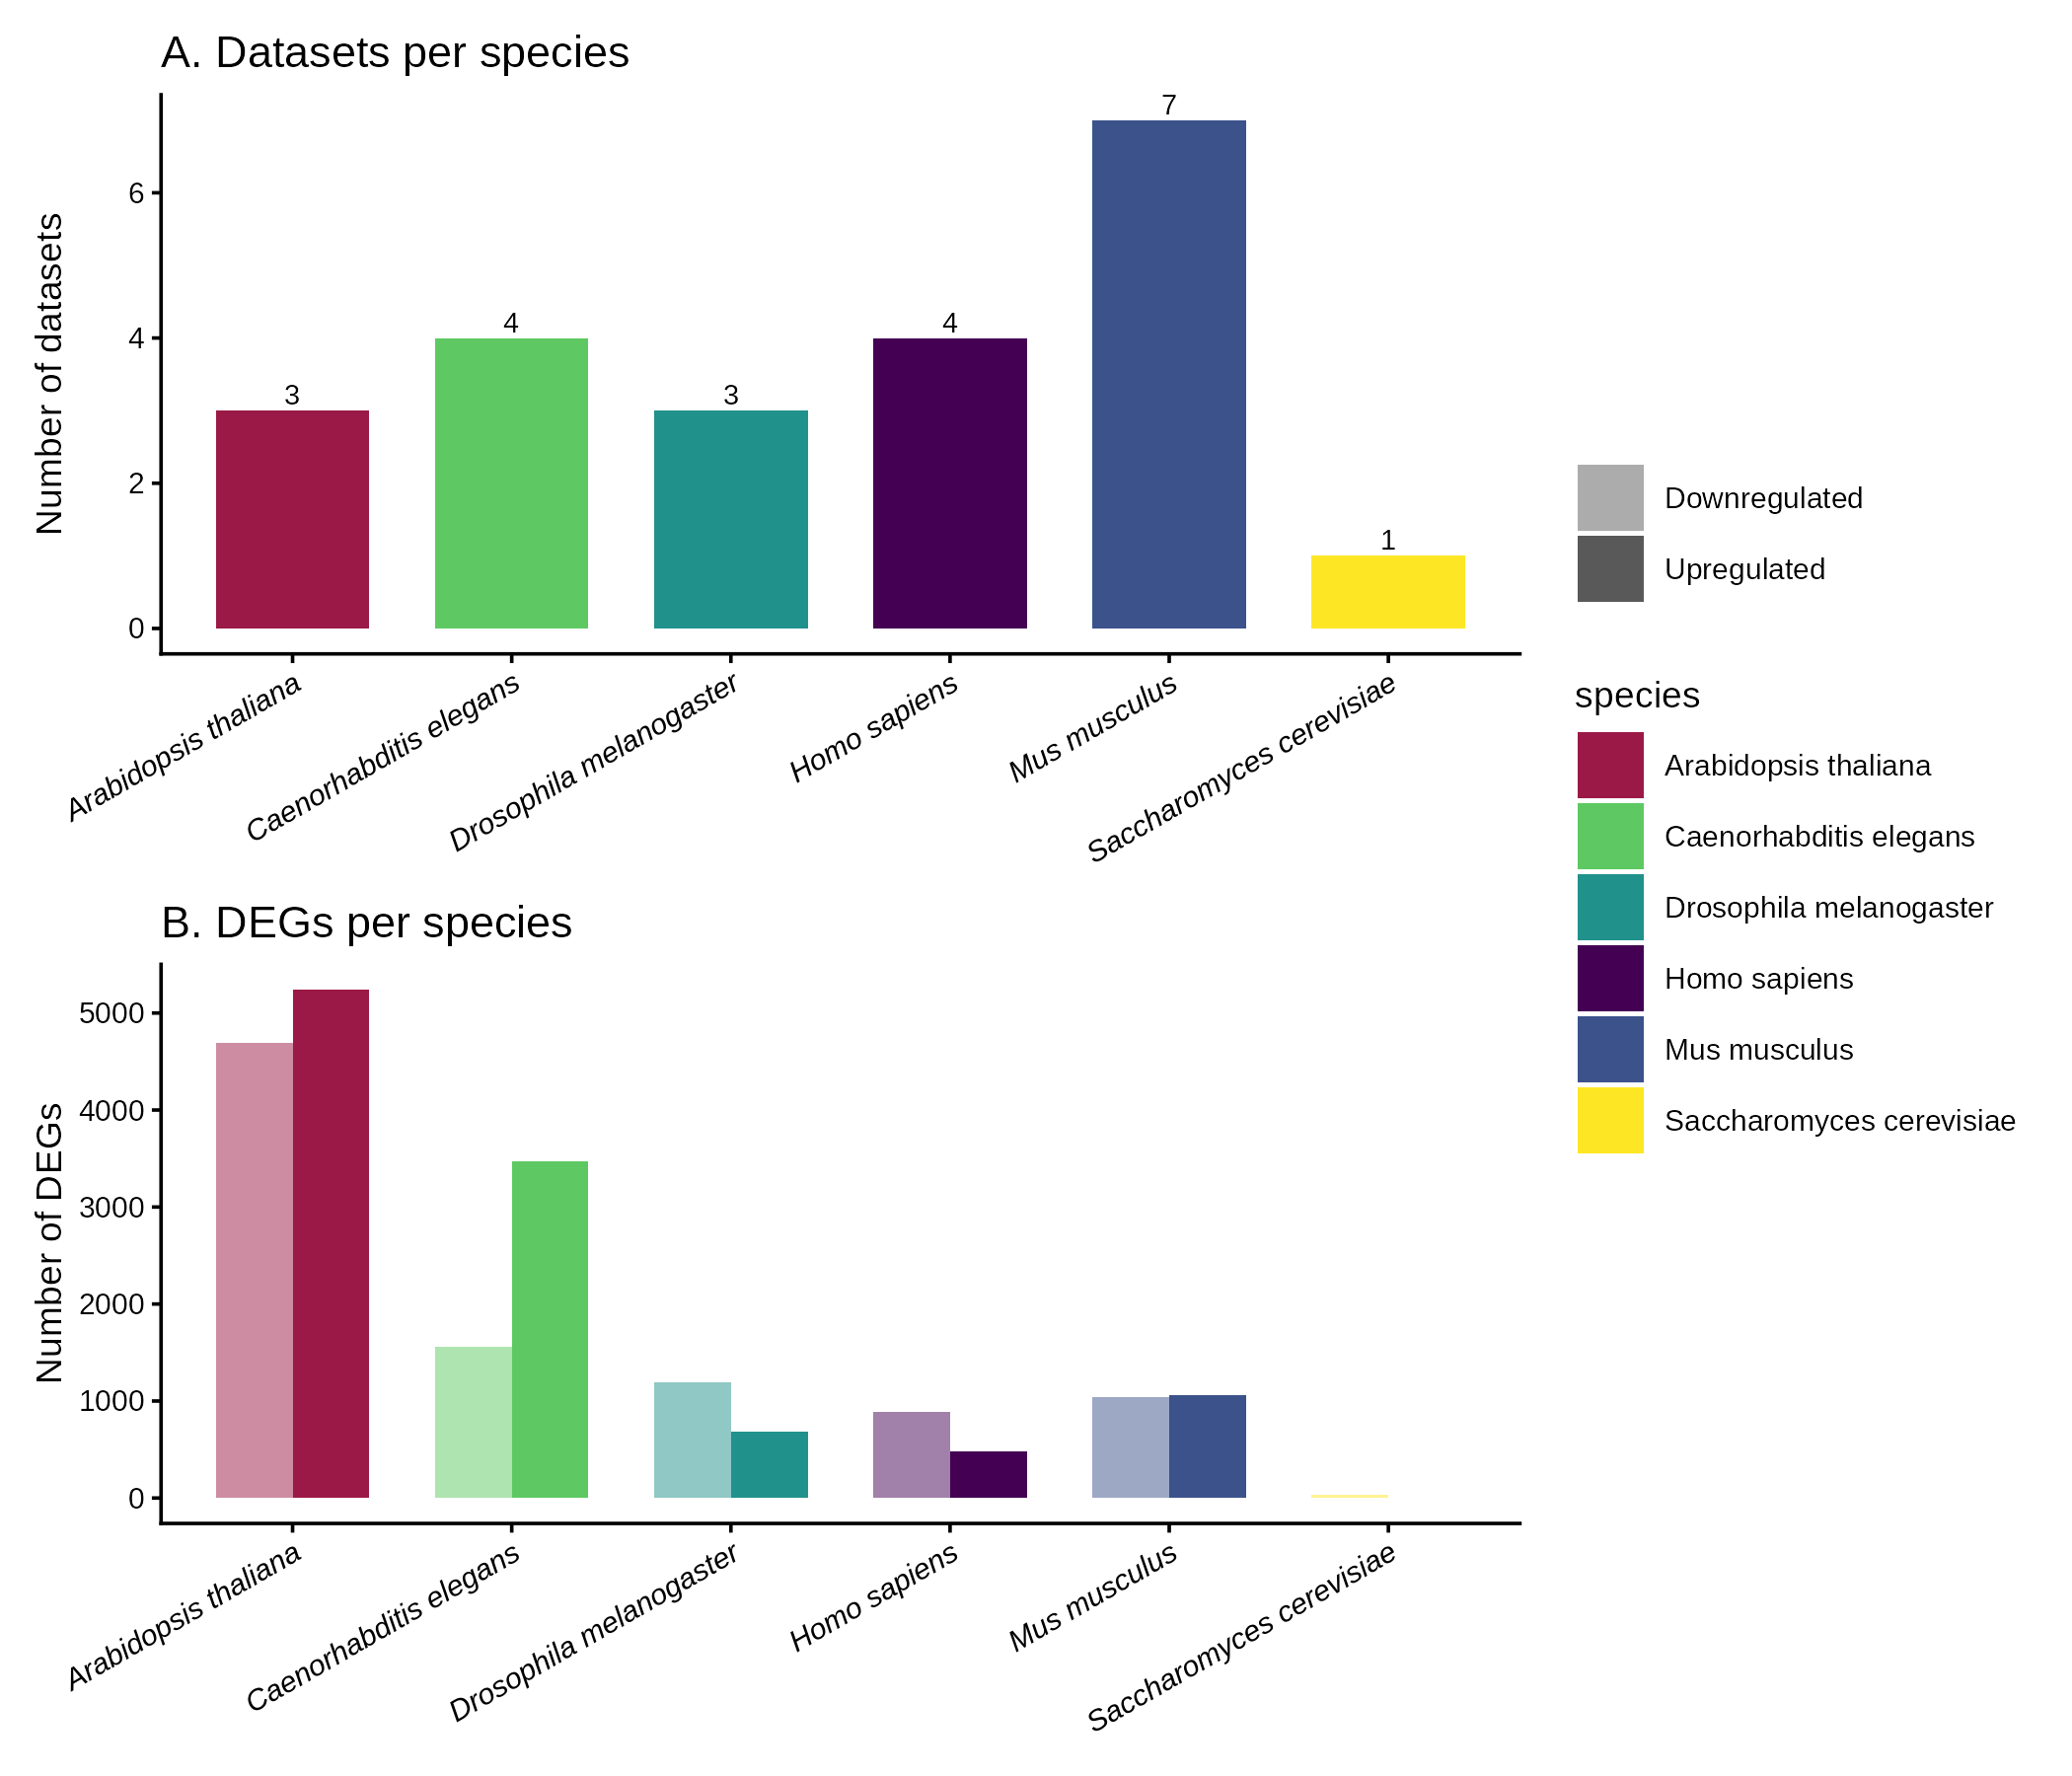
\includegraphics[width=0.9\textwidth]{fig1_study_overview.png}
    \caption{
        \textbf{Study overview and dataset composition.}
        (a) Schematic of the cross-species meta-analysis workflow.
        (b) Dataset counts per species showing RNA-seq (solid) and microarray (hatched) 
        studies. (c) Spaceflight duration (days) and tissue types across the 22 datasets.
        (d) Geographic and experimental facility distribution of datasets.
    }
    \label{fig:fig1}
\end{figure}

\subsection{Per-species differential expression and volcano plots}
\label{sec:results:volcano}

\cref{fig:fig2} displays volcano plots for each species showing the log$_2$ fold change 
and statistical significance of all expressed genes. The number and magnitude of 
spaceflight-induced changes vary across species, reflecting differences in mission 
duration, tissue sampled, and organismal physiology. Despite this heterogeneity, 
all species show a characteristic pattern: both upregulated and downregulated genes 
are observed, but certain functional categories (notably mitochondrial and metabolic 
genes) appear consistently suppressed across multiple species.

\begin{figure}[h]
    \centering
    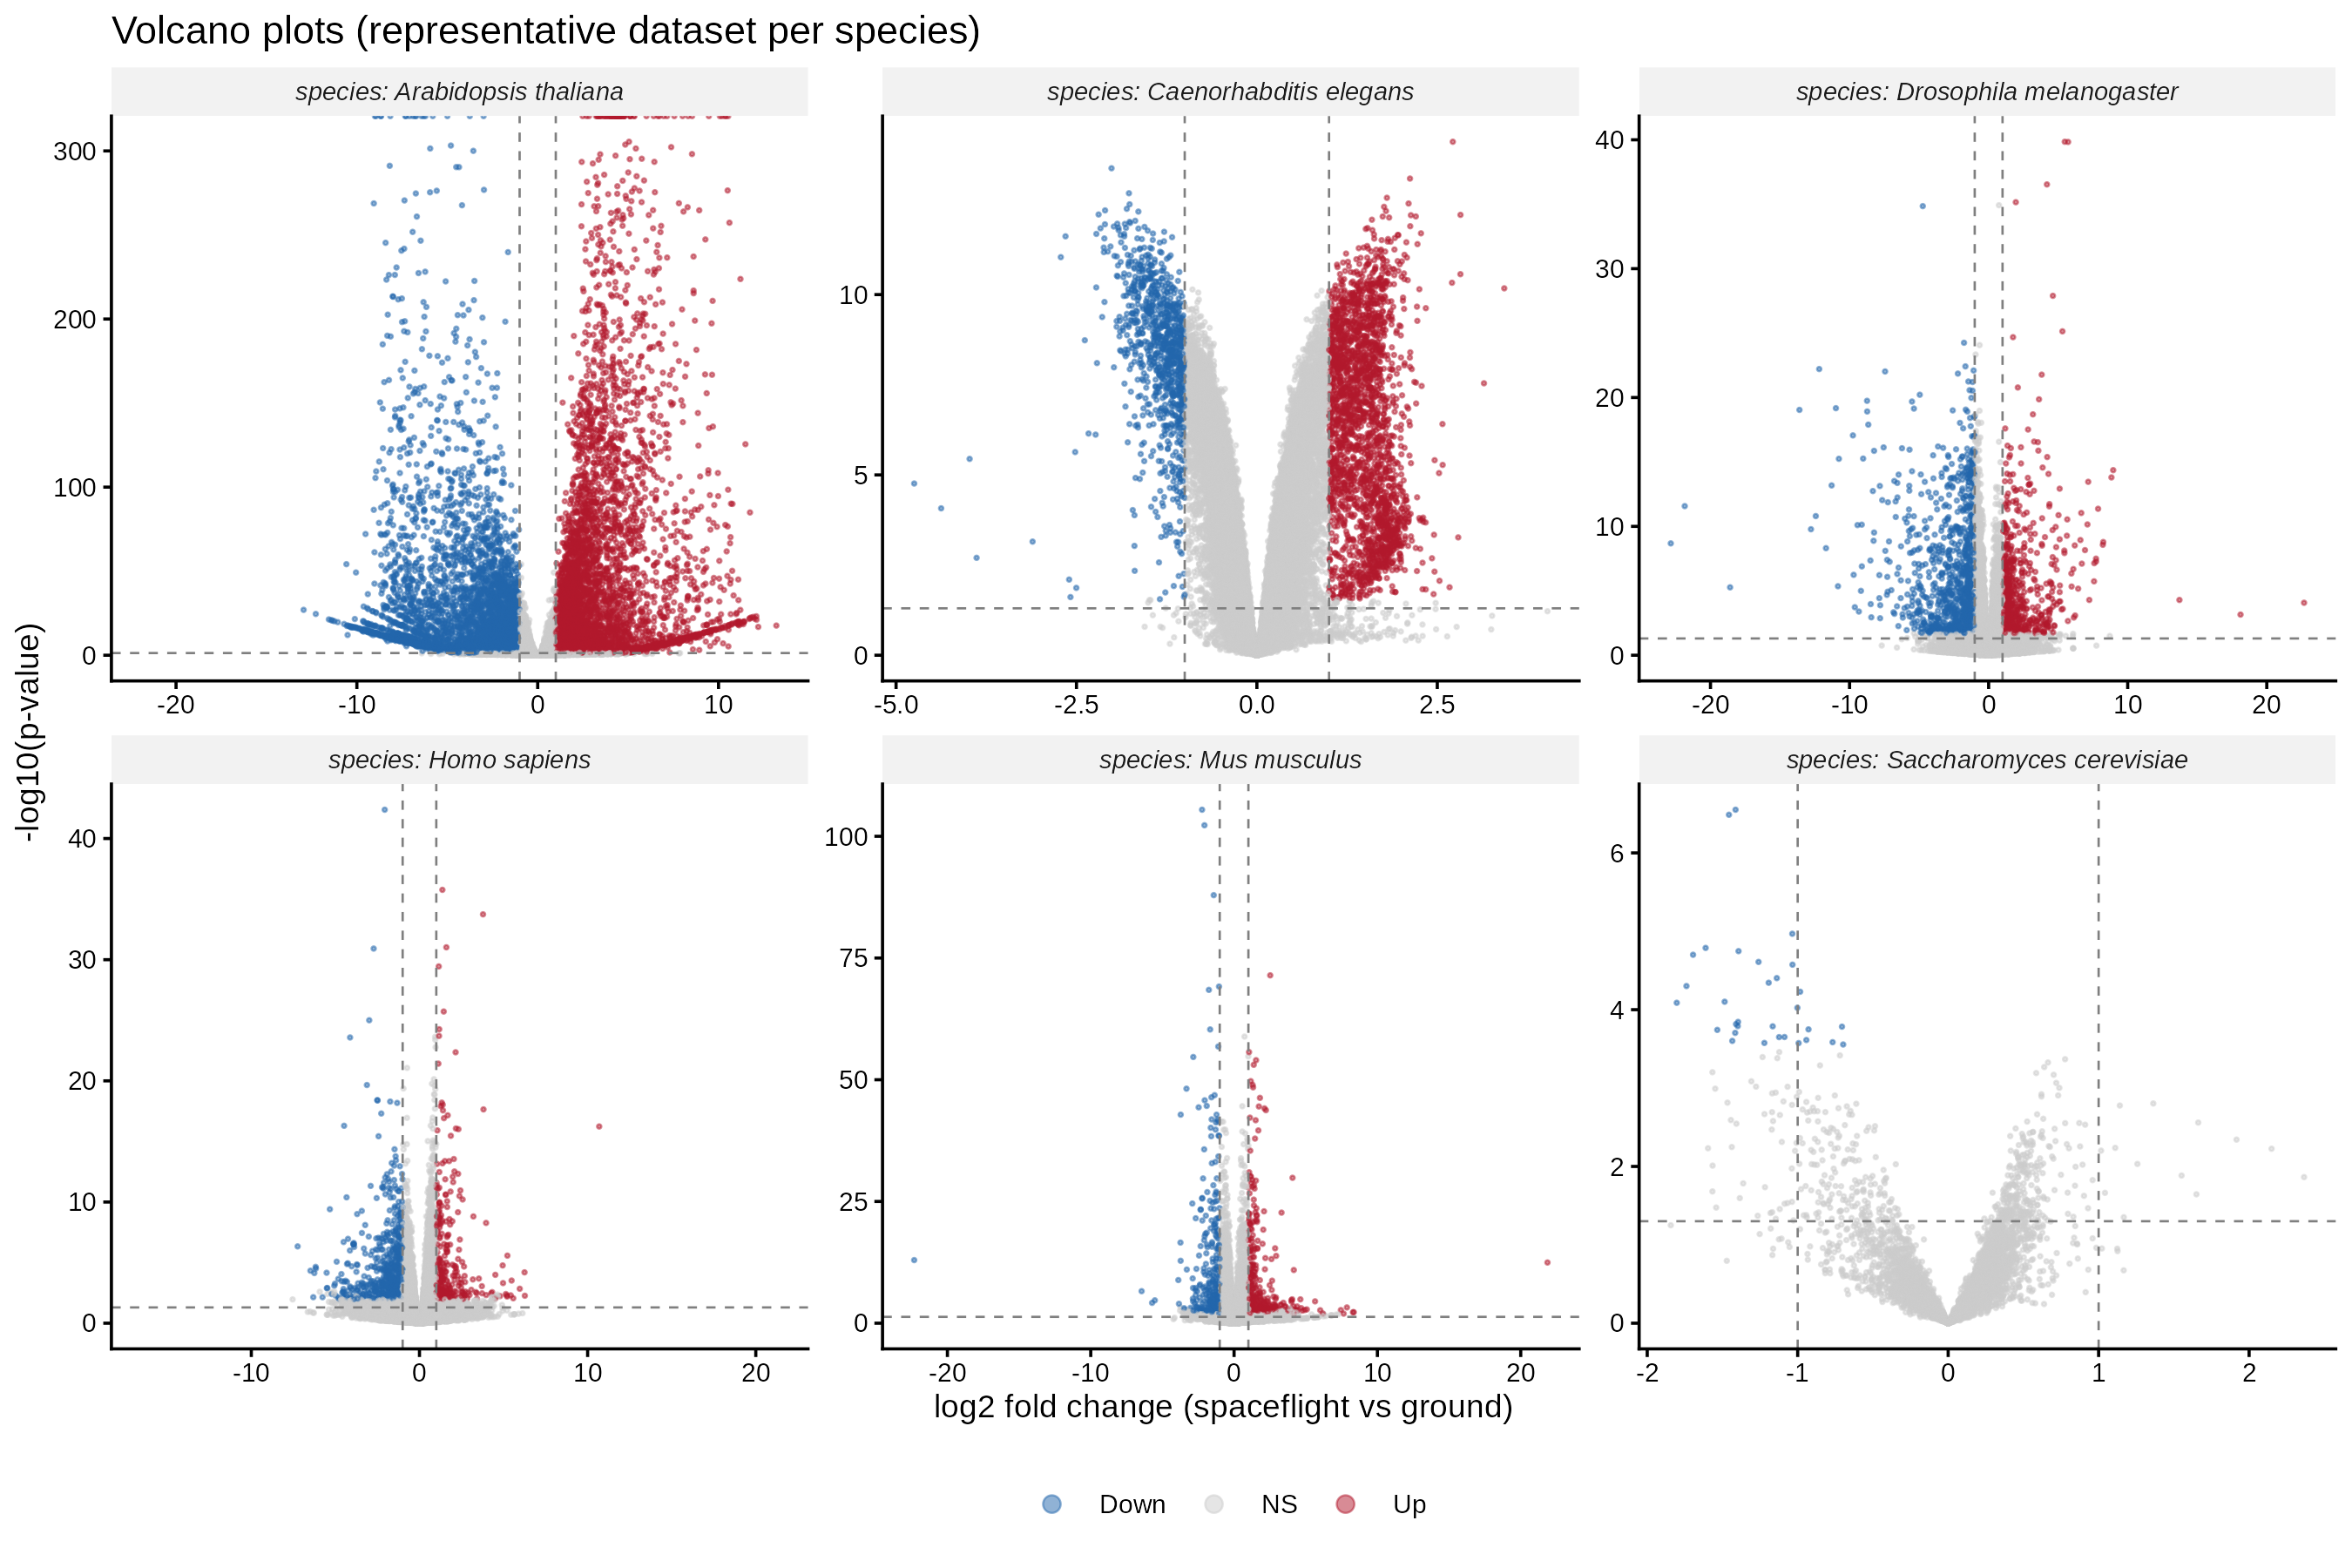
\includegraphics[width=1.0\textwidth]{fig2_volcano_plots.png}
    \caption{
        \textbf{Per-species differential expression volcano plots.}
        Each panel shows $-\log_{10}$(adjusted $p$-value) versus $\log_2$(fold change) 
        for all genes in each species. Colors indicate direction of change: red, upregulated; 
        blue, downregulated. Horizontal dashed line marks padj $= 0.05$. Vertical dashed 
        lines mark $|\log_2\text{FC}| = 1$.
    }
    \label{fig:fig2}
\end{figure}

\subsection{Orthology mapping and cross-species alignment}
\label{sec:results:orthology}

To identify conserved responses, we mapped genes across species using a human-anchored 
orthology matrix built from OrthoDB v12. This matrix contains 51,474 ortholog pairs 
covering 18,030 human genes, of which 651 have orthologs in all six target species.

\cref{fig:fig3} shows the overlaps in orthologous gene membership across the six species. 
The vast majority of DEGs map to orthologs in other species (e.g., 76\% of mouse DEGs 
have human orthologs), but only a small fraction (651 genes) have representatives in all 
six species. This orthology distribution reflects the evolutionary distances between 
species and influences the statistical power to detect cross-species conservation.

\begin{figure}[h]
    \centering
    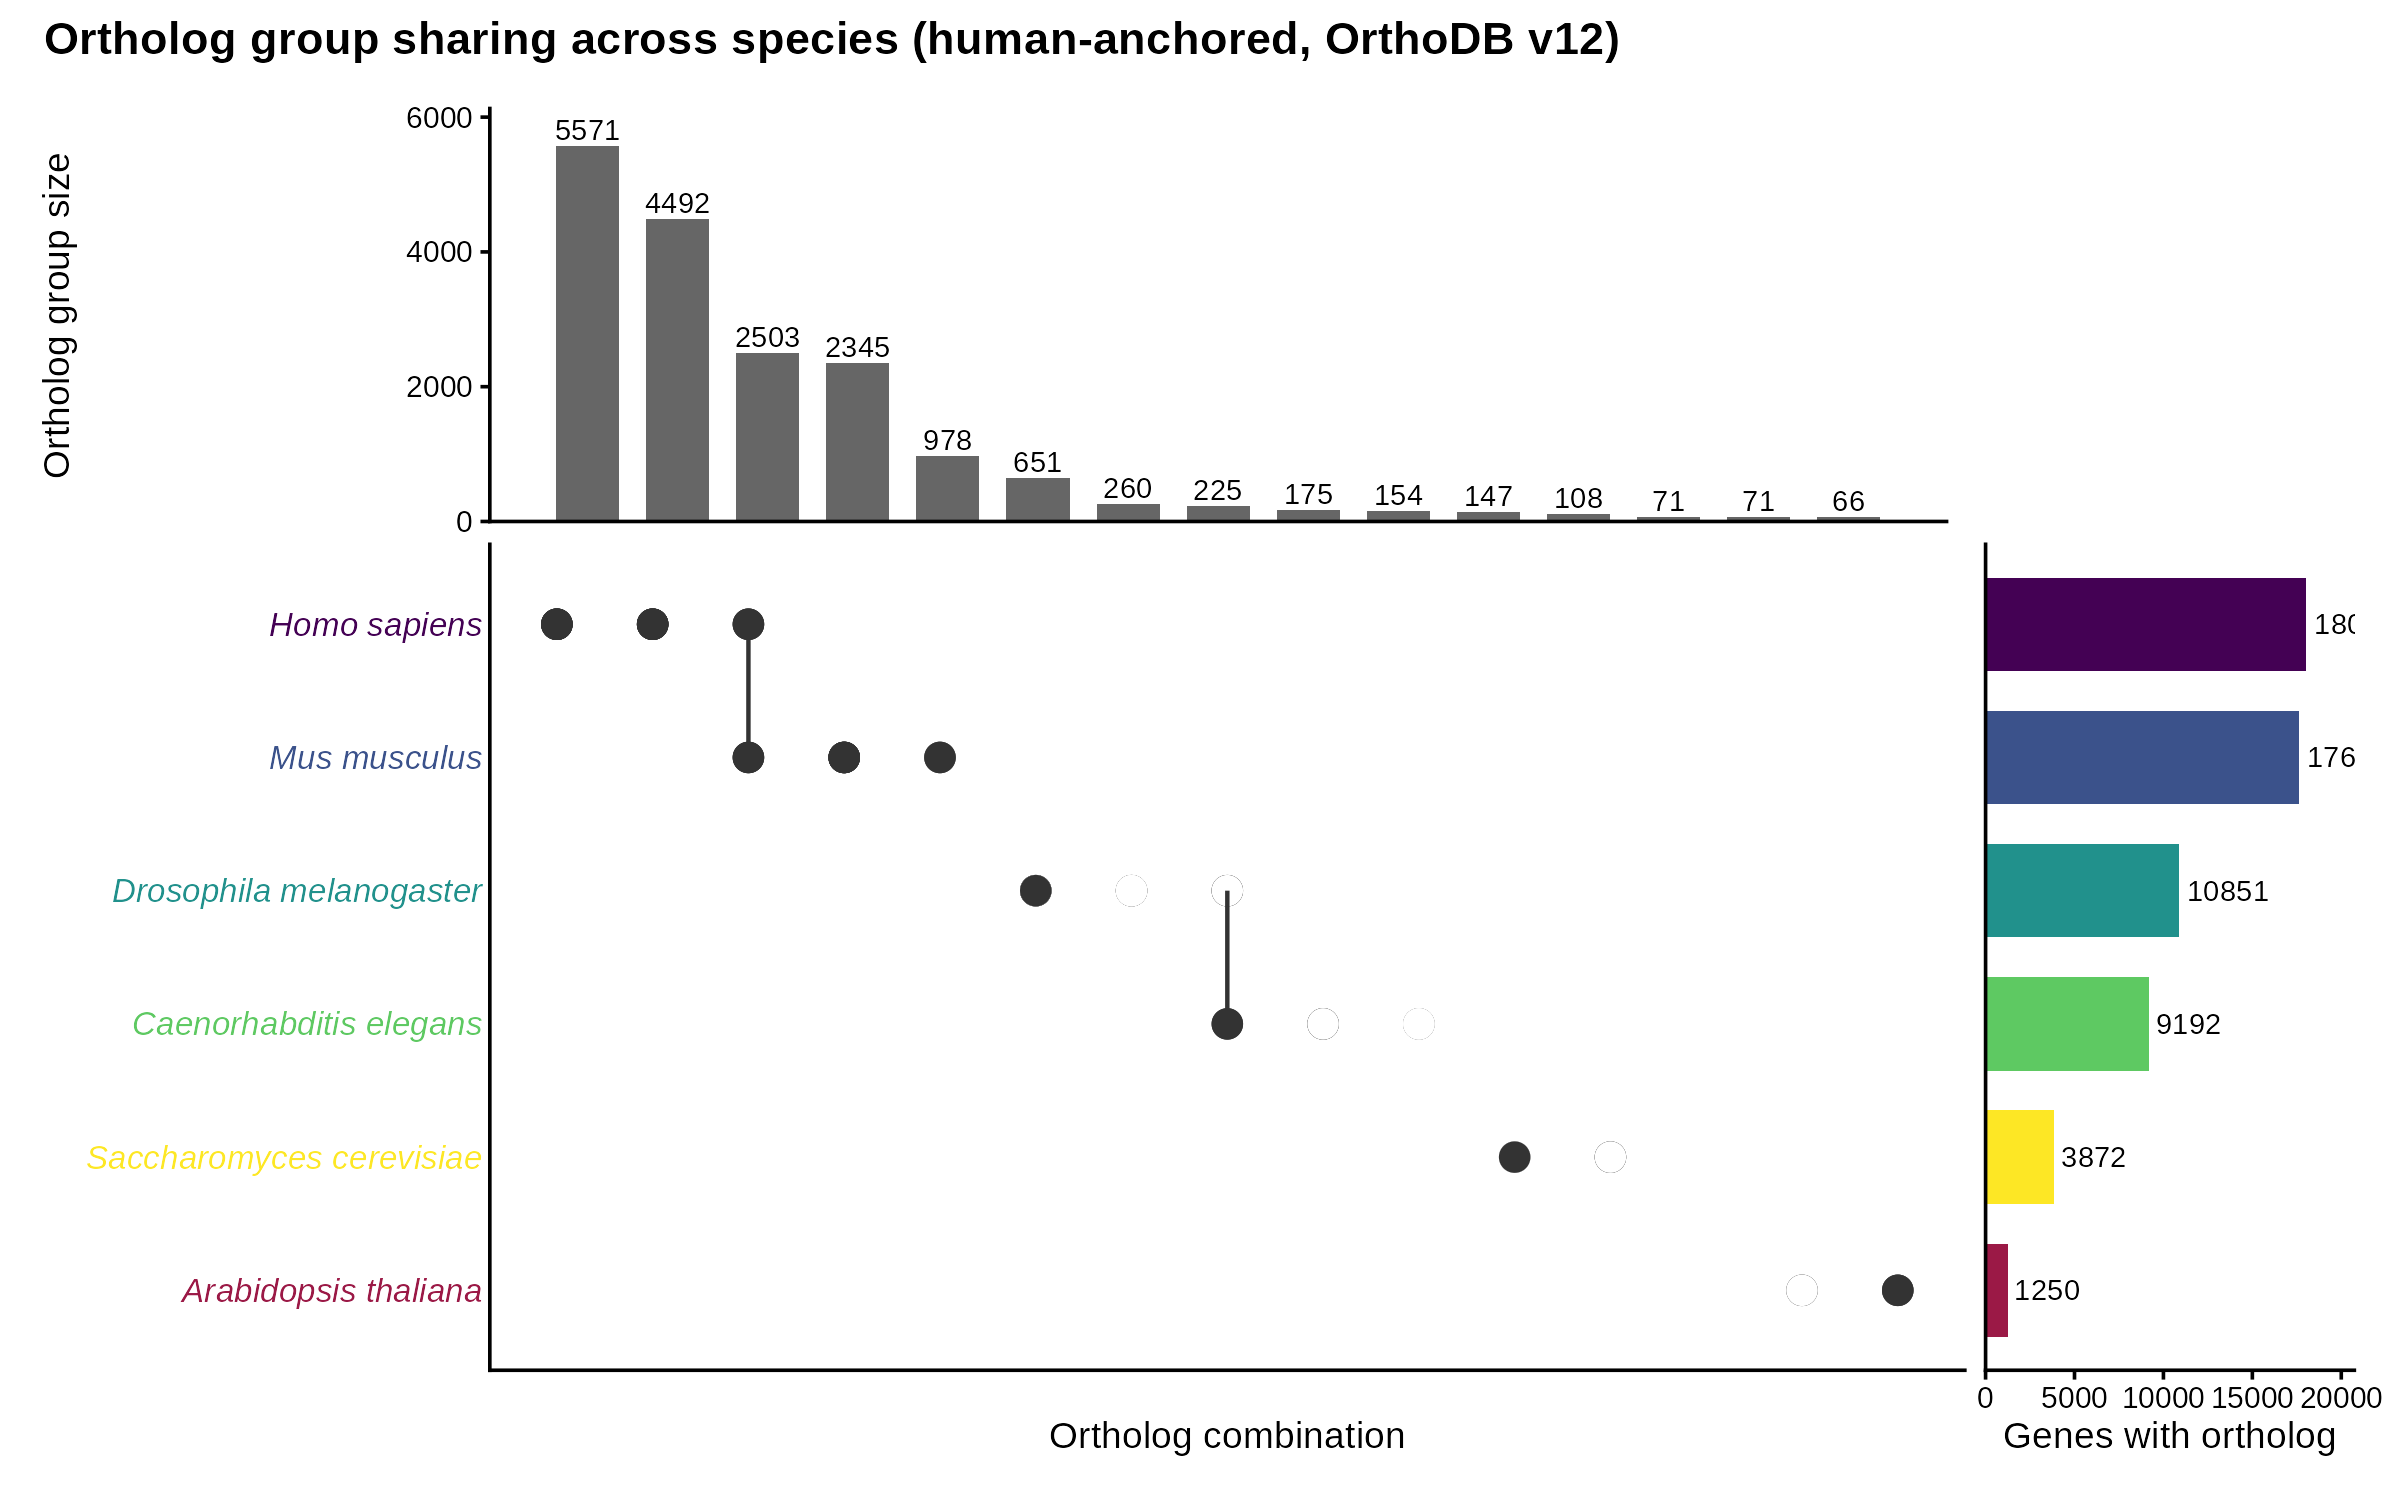
\includegraphics[width=0.75\textwidth]{fig3_orthology_upset.png}
    \caption{
        \textbf{Ortholog sharing across species (UpSet plot).}
        Intersection sizes show the number of human-anchored orthologs detected as DEGs 
        in each species combination. The most populated intersections are those involving 
        human, mouse, and fly (evolutionary proximity). The small intersection at the 
        right (all six species) comprises the 651 orthologs with representatives in all 
        target species—these are the most powerful for cross-species detection.
    }
    \label{fig:fig3}
\end{figure}

\subsection{Subcellular compartment enrichment and conservation}
\label{sec:results:enrichment}

We assigned all DEGs to 16 subcellular compartments (Cell wall/ECM, Plasma membrane, 
Extracellular, Cytoskeleton, Nucleus, Proteasome, Ribosome, Mitochondrion, Membrane 
transport, Lysosome, Endosome, Peroxisome, ER/Golgi, Cytosol, Chromatin, Other) based 
on Gene Ontology Cellular Component (GO CC) enrichment. For each compartment, we applied 
Fisher's combined probability test to detect organelles with direction-consistent, 
cross-species DE signal.

\cref{fig:fig4} displays a heatmap of compartment-level conservation, with colors 
indicating the mean log$_2$ fold change of genes assigned to each compartment in each 
species. The most striking pattern is the pervasive blue coloring of the mitochondrial 
row—indicating consistent downregulation across all six species. Other organelles show 
more heterogeneous patterns, with some showing species-specific or tissue-specific 
responses.

\begin{figure}[h]
    \centering
    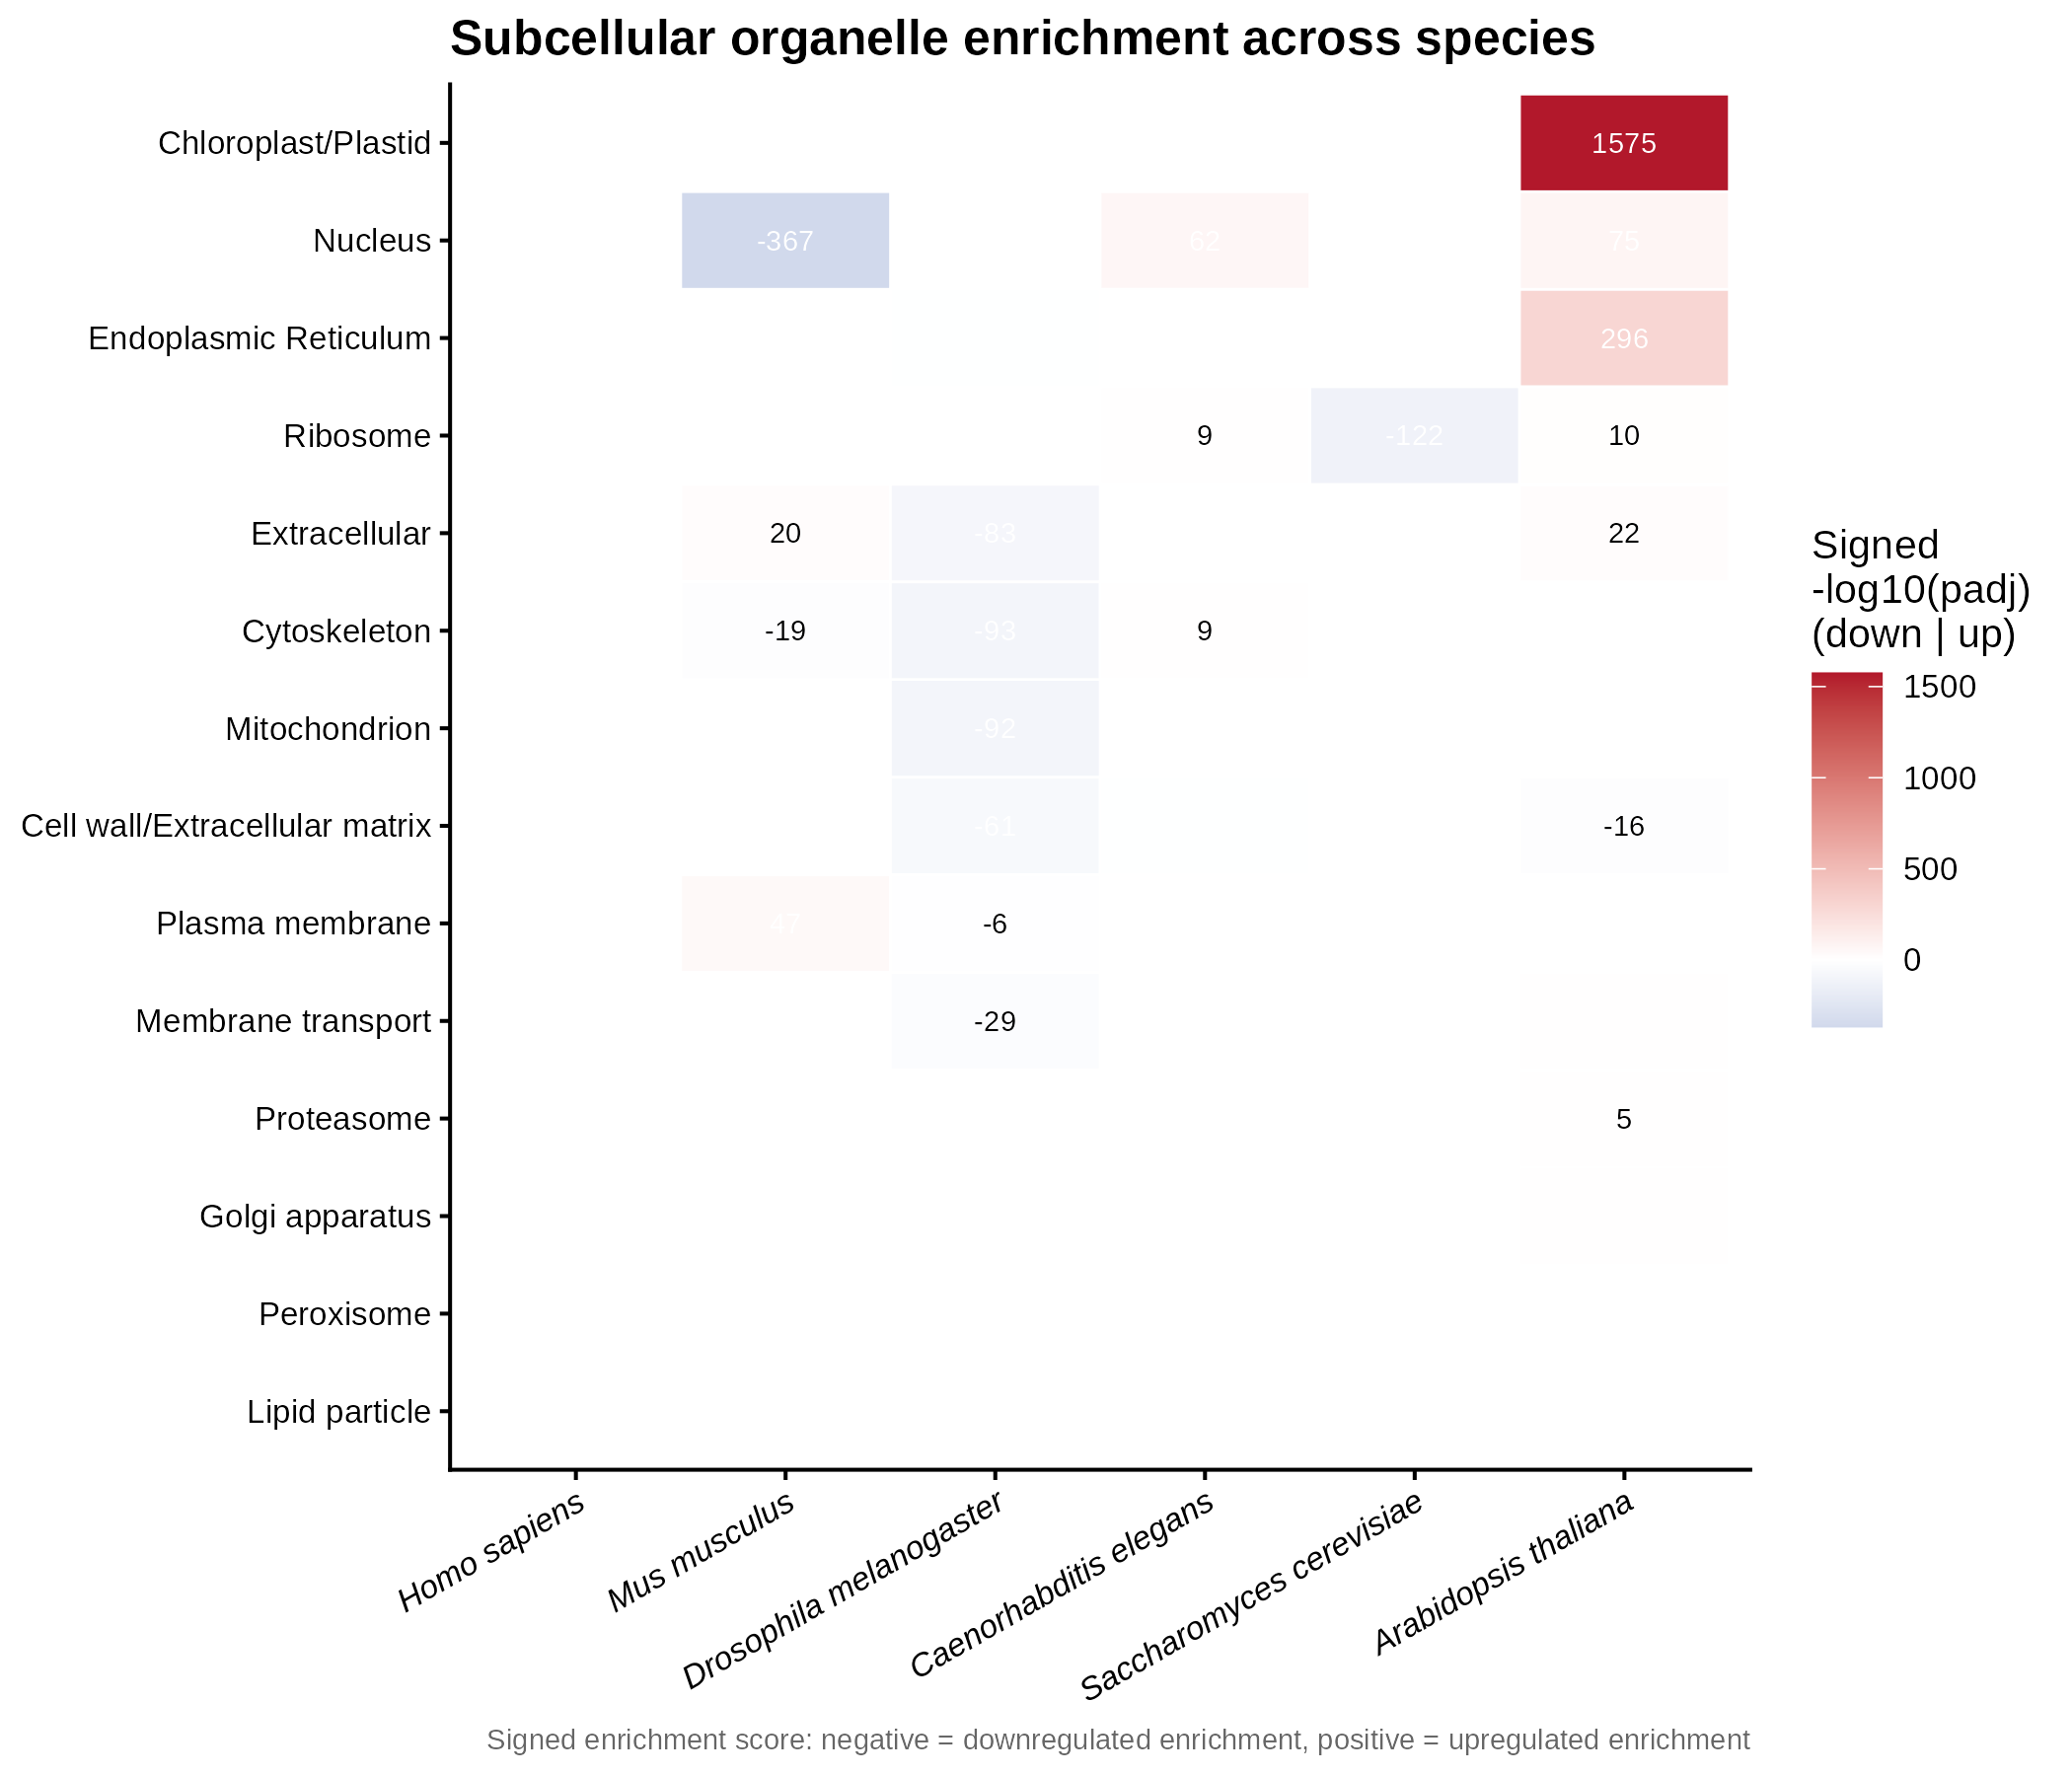
\includegraphics[width=1.0\textwidth]{fig4_organelle_enrichment_heatmap.png}
    \caption{
        \textbf{Organelle-level conservation heatmap.}
        Rows represent 16 subcellular compartments; columns represent the six species. 
        Color intensity and direction indicate mean $\log_2$(fold change) of genes in each 
        compartment (red, upregulated; blue, downregulated). Asterisks denote compartments 
        with FDR $< 0.05$ by Fisher's combined test. The mitochondrial row shows 
        consistent downregulation across all species.
    }
    \label{fig:fig4}
\end{figure}

\subsection{Conserved mitochondrial suppression: Orthologs and pathways}
\label{sec:results:mito}

The most significant finding of this meta-analysis is the identification of 49 
mitochondrial orthologs showing direction-consistent downregulation across at least 
three species (adjusted Fisher $p < 0.05$, $\geq 80\%$ direction consistency). 
These genes encode components of critical mitochondrial processes: oxidative 
phosphorylation (electron transport chain, ATP synthase), the TCA cycle, fatty acid 
oxidation, and amino acid metabolism.

\cref{fig:fig5} presents a schematic representation of mitochondrial compartments 
and the conserved suppression pattern. Matrix enzymes, inner membrane complexes, 
and cristae-associated proteins all show suppression, suggesting that spaceflight 
induces a broad, coordinated downregulation of mitochondrial metabolic capacity.

\begin{figure}[h]
    \centering
    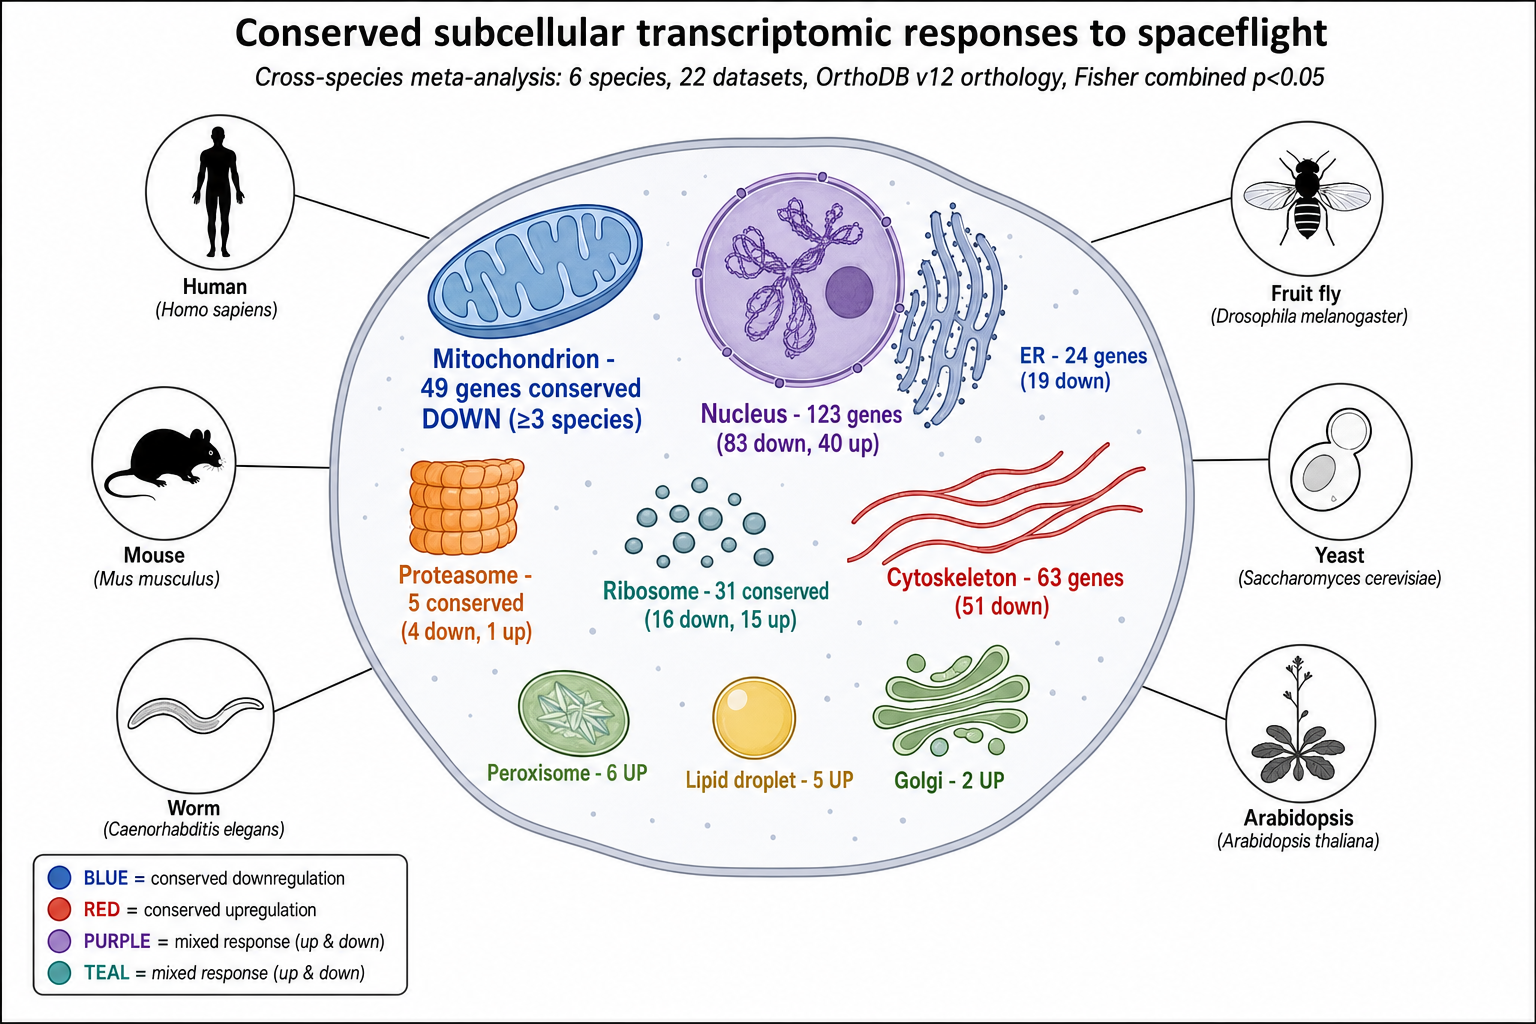
\includegraphics[width=0.85\textwidth]{fig5_conserved_organelle_schematic.png}
    \caption{
        \textbf{Schematic of conserved mitochondrial suppression.}
        Cartoon cross-section of a mitochondrion showing major structural and functional 
        compartments. Text annotations (with gene symbols) highlight the conserved 
        downregulated orthologs in each region: outer membrane, intermembrane space, 
        inner membrane (ETC, ATP synthase), and matrix (TCA cycle, amino acid metabolism).
    }
    \label{fig:fig5}
\end{figure}

To validate this ortholog-level finding at the pathway level, we interrogated four 
KEGG pathways enriched in the mitochondrial-suppressed gene set: TCA cycle (hsa00020), 
oxidative phosphorylation (hsa00190), ribosome (hsa03010), and proteasome (hsa03050). 
\cref{fig:fig6} displays per-species pathway diagrams with overlaid $\log_2$(fold change) 
values for each gene across the six species.

\begin{figure}[h]
    \centering
    \begin{subfigure}{\textwidth}
        \centering
        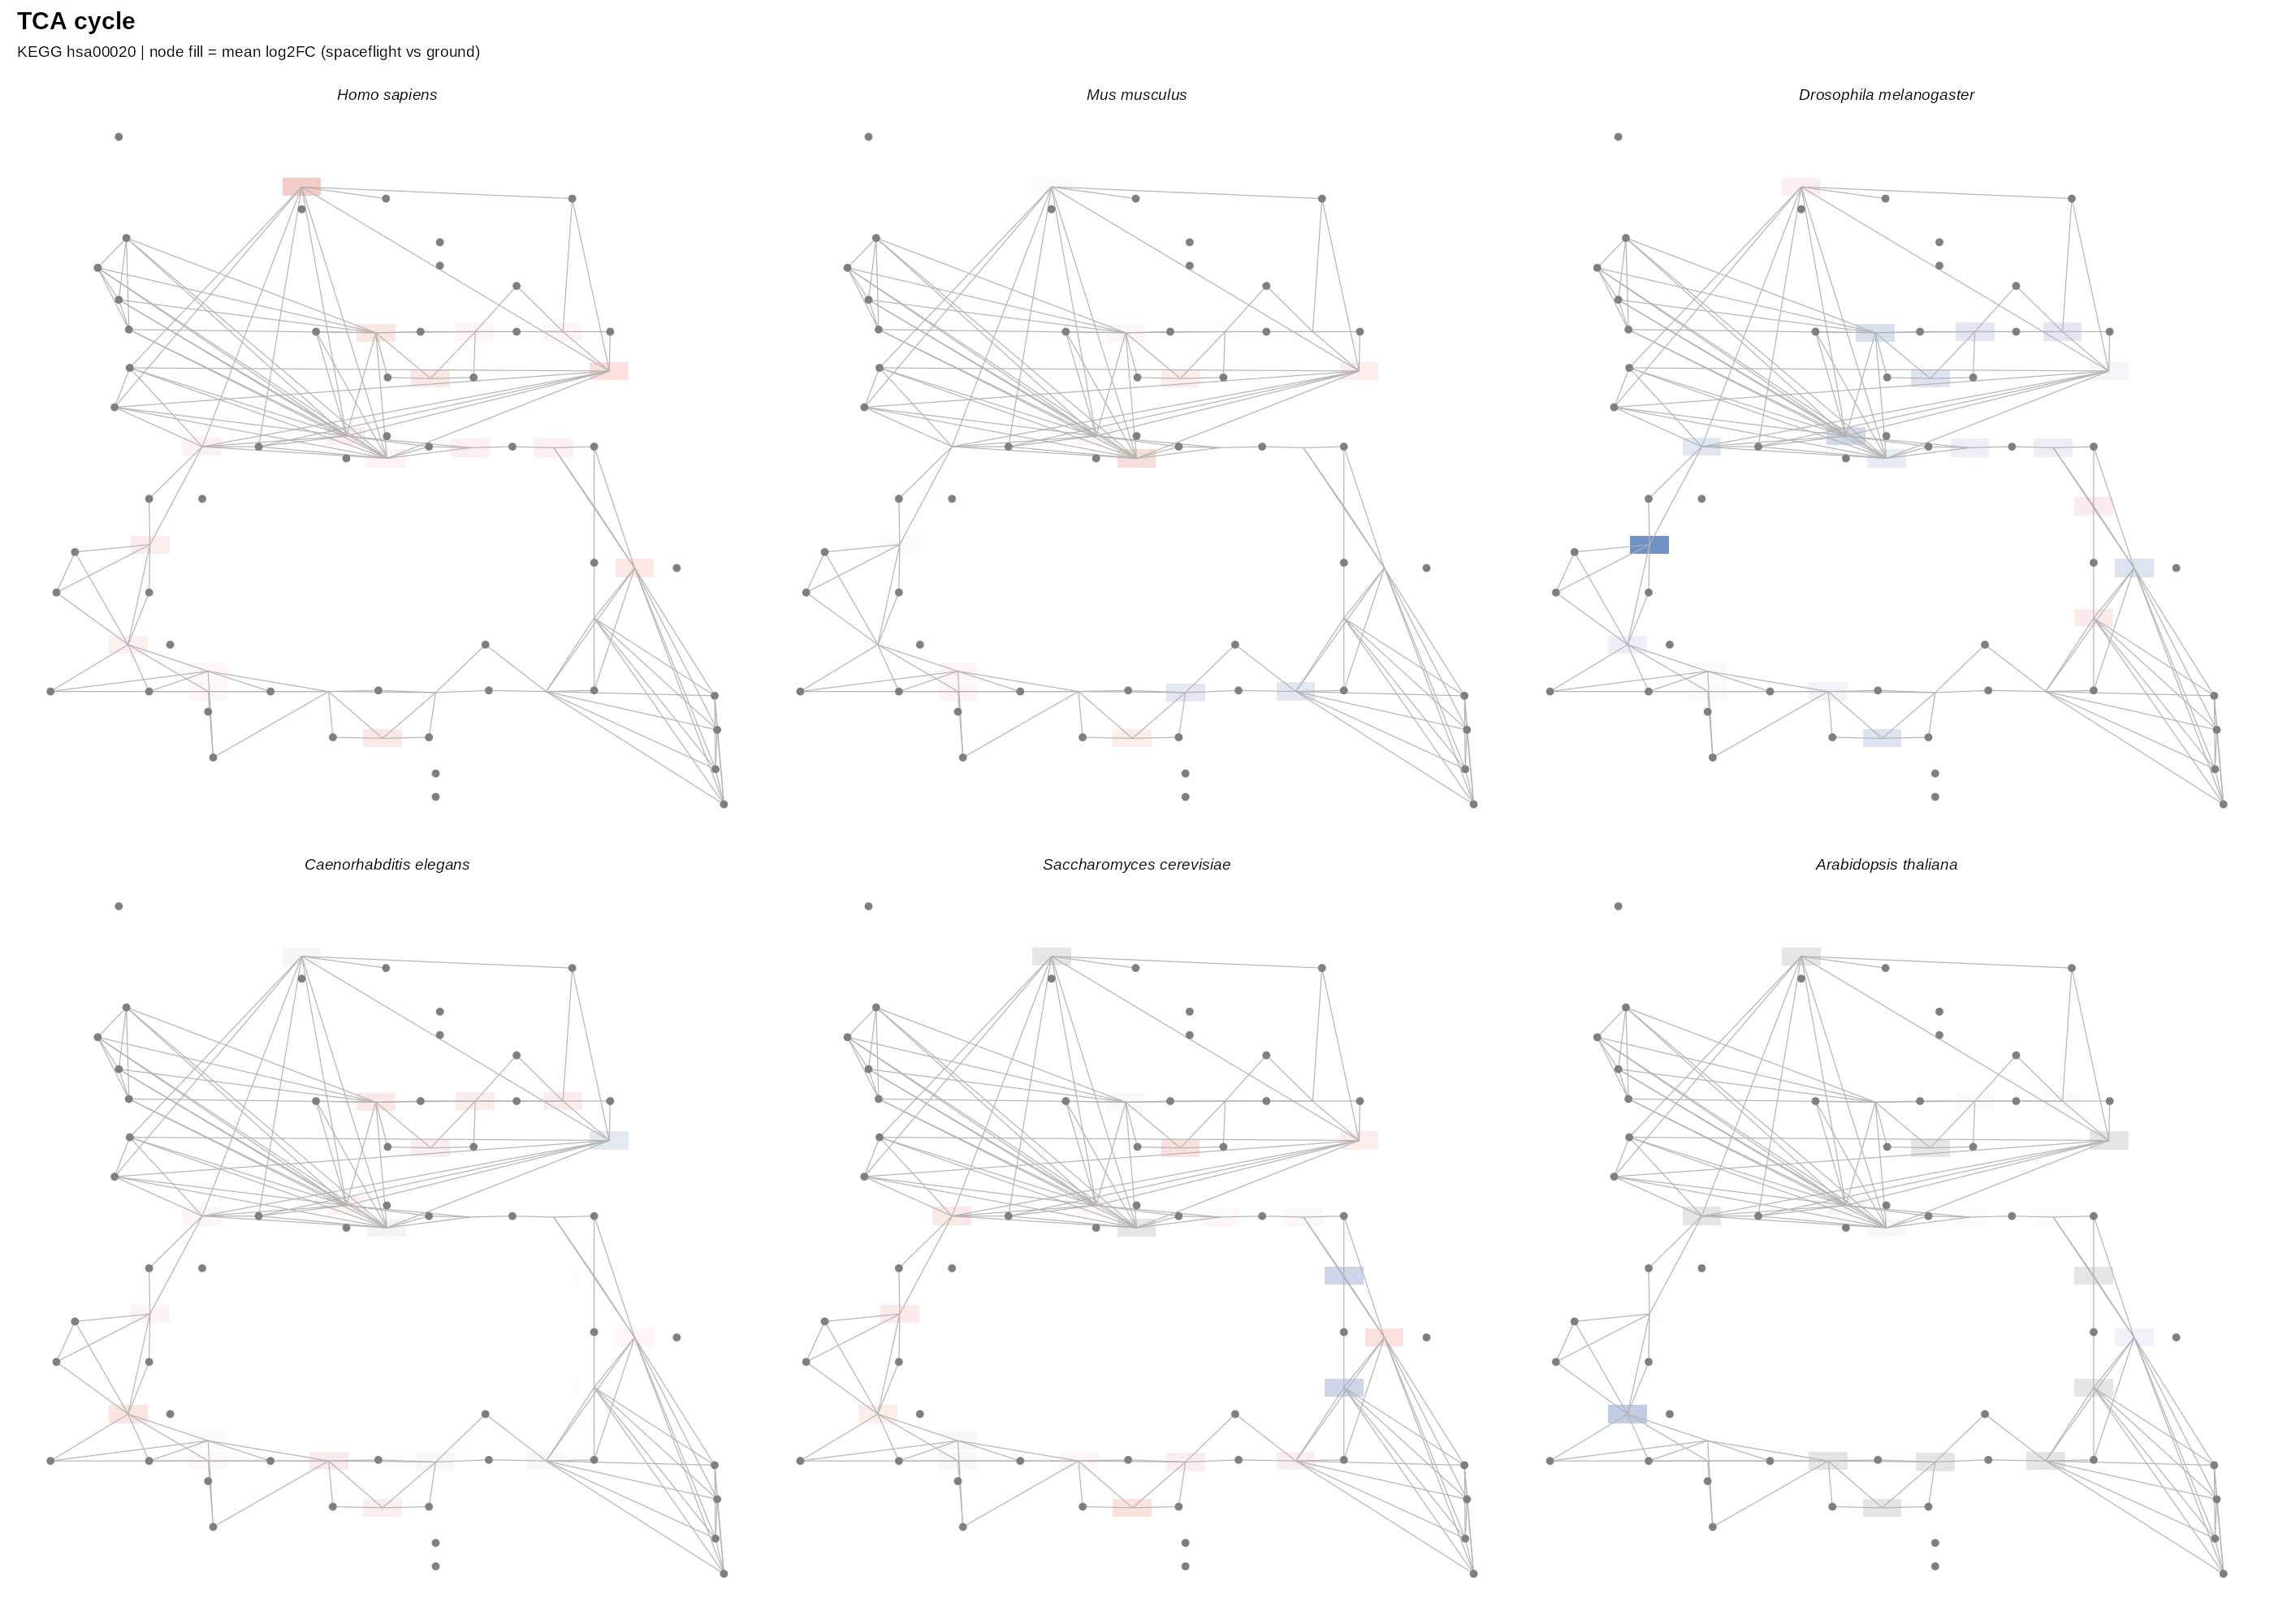
\includegraphics[width=0.95\textwidth]{fig6_pathway_hsa00020.png}
        \caption{TCA cycle (hsa00020)}
    \end{subfigure}
    \begin{subfigure}{\textwidth}
        \centering
        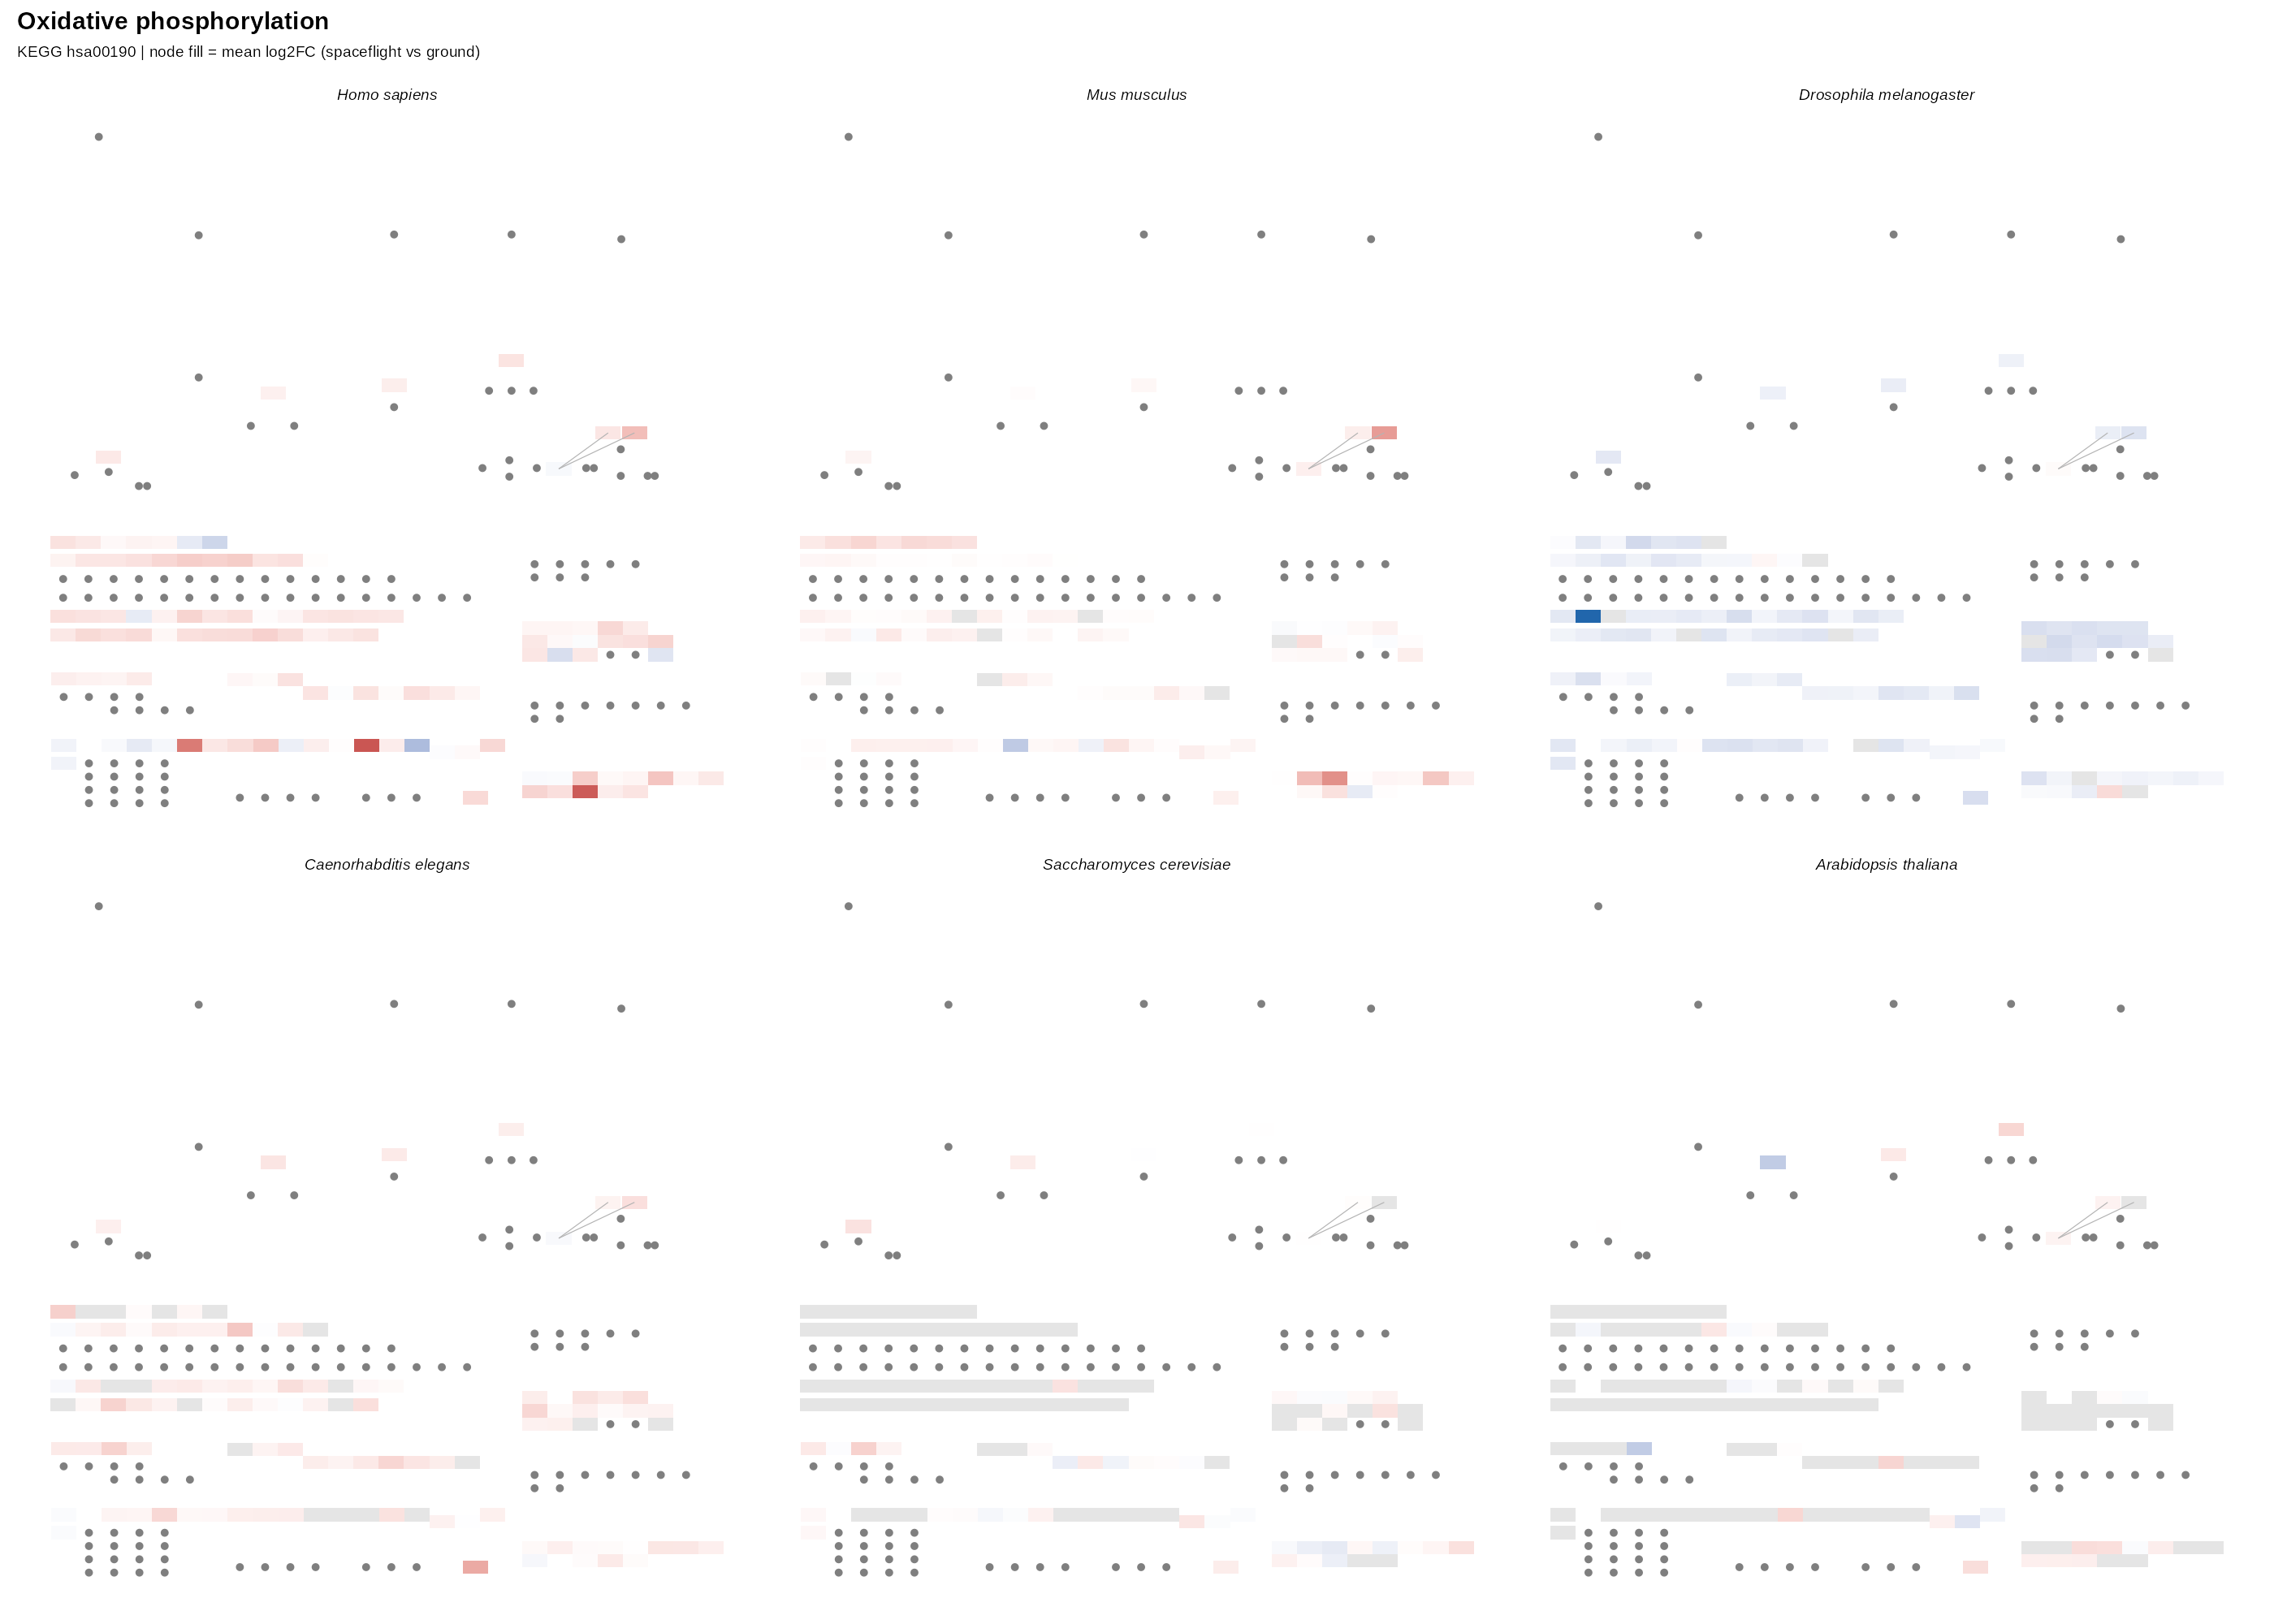
\includegraphics[width=0.95\textwidth]{fig6_pathway_hsa00190.png}
        \caption{Oxidative phosphorylation (hsa00190)}
    \end{subfigure}
    \begin{subfigure}{\textwidth}
        \centering
        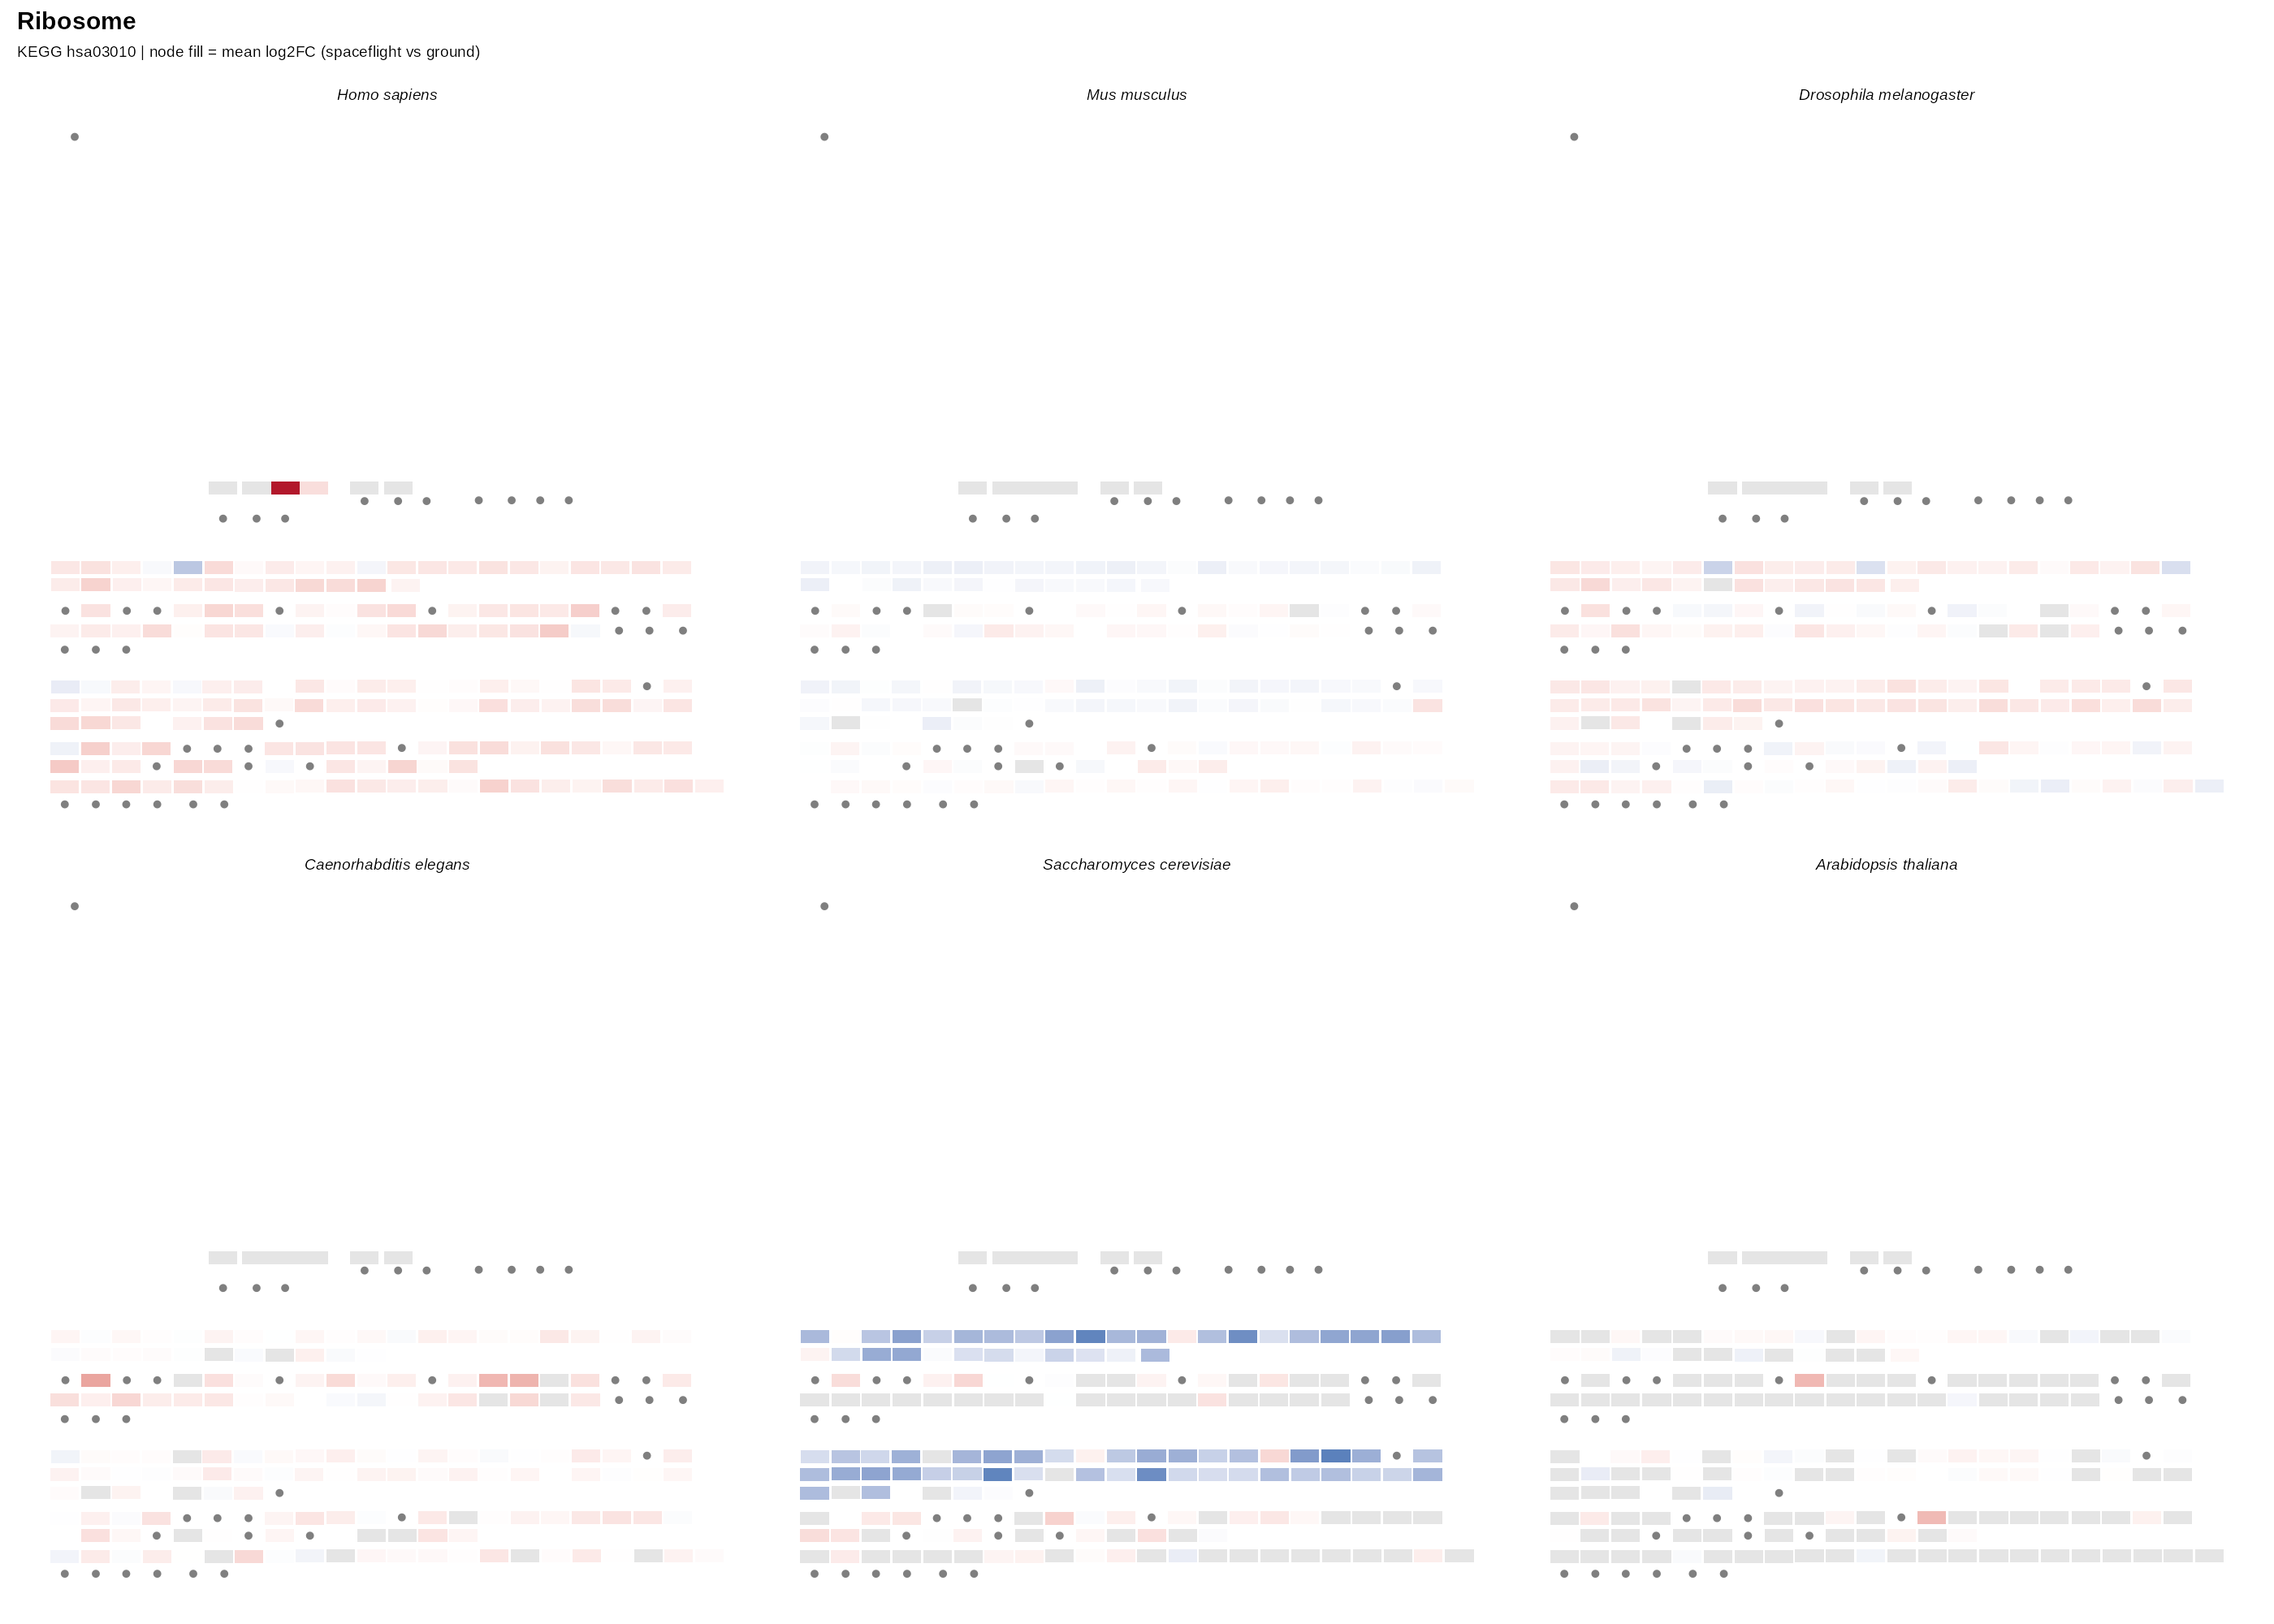
\includegraphics[width=0.95\textwidth]{fig6_pathway_hsa03010.png}
        \caption{Ribosome (hsa03010)}
    \end{subfigure}
    \begin{subfigure}{\textwidth}
        \centering
        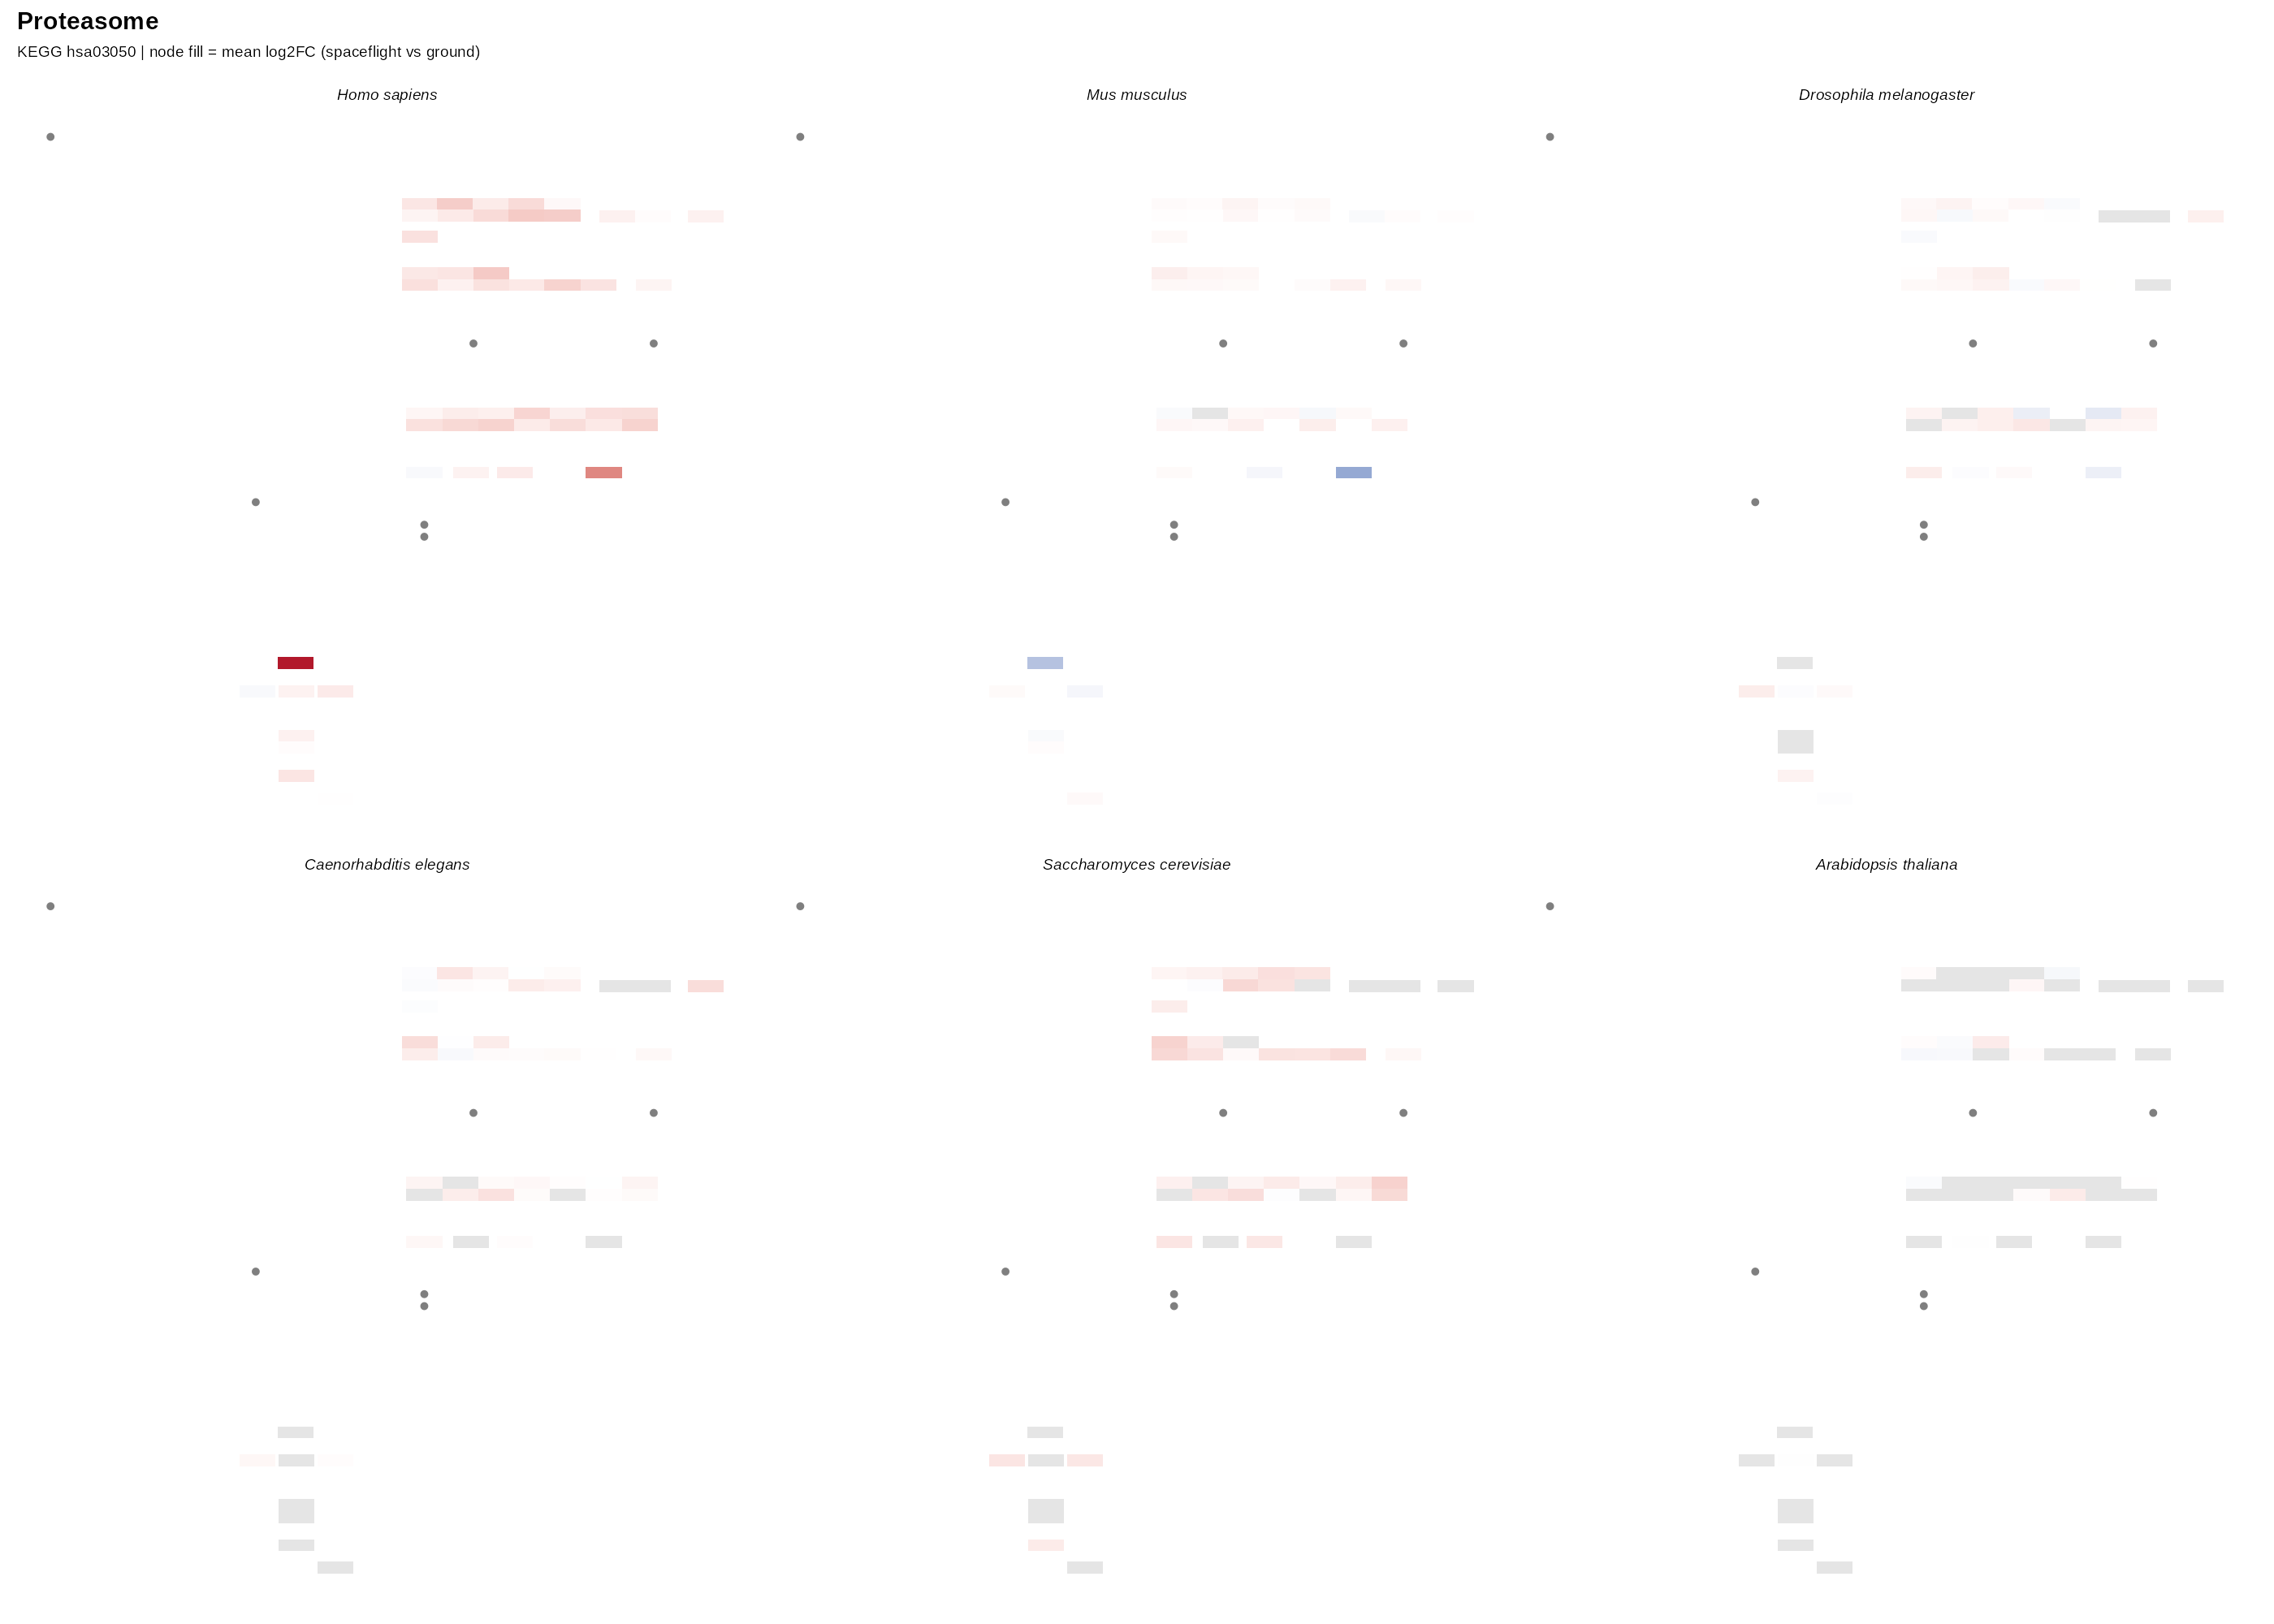
\includegraphics[width=0.95\textwidth]{fig6_pathway_hsa03050.png}
        \caption{Proteasome (hsa03050)}
    \end{subfigure}
    \caption{
        \textbf{KEGG pathway analysis with per-species fold changes.}
        Each panel shows a KEGG pathway with nodes (genes) colored by mean $\log_2$(FC) 
        across all six species. (a) TCA cycle genes show predominantly blue (downregulated) 
        coloring. (b) Oxidative phosphorylation (ETC and ATP synthase) similarly shows 
        consistent downregulation. (c) Ribosomal and (d) proteasomal genes show more 
        heterogeneous responses, suggesting that protein synthesis and degradation are 
        less universally affected.
    }
    \label{fig:fig6}
\end{figure}

\subsection{Cofactor enrichment: NAD+, FAD, and heme}
\label{sec:results:cofactors}

We hypothesized that the conserved downregulation of mitochondrial metabolic genes 
would be reflected in reduced expression of genes encoding cofactors essential for 
mitochondrial electron transport and TCA cycle function. We mapped 14 enzyme cofactors 
(NAD+, NADH, NADP+, NADPH, FAD, FADH2, FMN, CoA, TPP, Lipoamide, Biotin, Heme, 
and attempted Fe-S clusters and Zn$^{2+}$) to human genes using KEGG compound-reaction-enzyme-gene 
chains, yielding 498 unique genes across 12 cofactors.

\cref{fig:fig7} summarizes the cofactor-gene enrichment findings. Genes involved in 
NAD+ biosynthesis and regeneration, FAD/FADH$_2$ handling, and heme synthesis/incorporation 
all show significant downregulation across multiple species, consistent with the reduced 
demand for electron transport and oxidative phosphorylation. This multi-level evidence—
orthologs, pathways, and cofactors—suggests a coordinated metabolic shift away from 
aerobic respiration in spaceflight.

\begin{figure}[h]
    \centering
    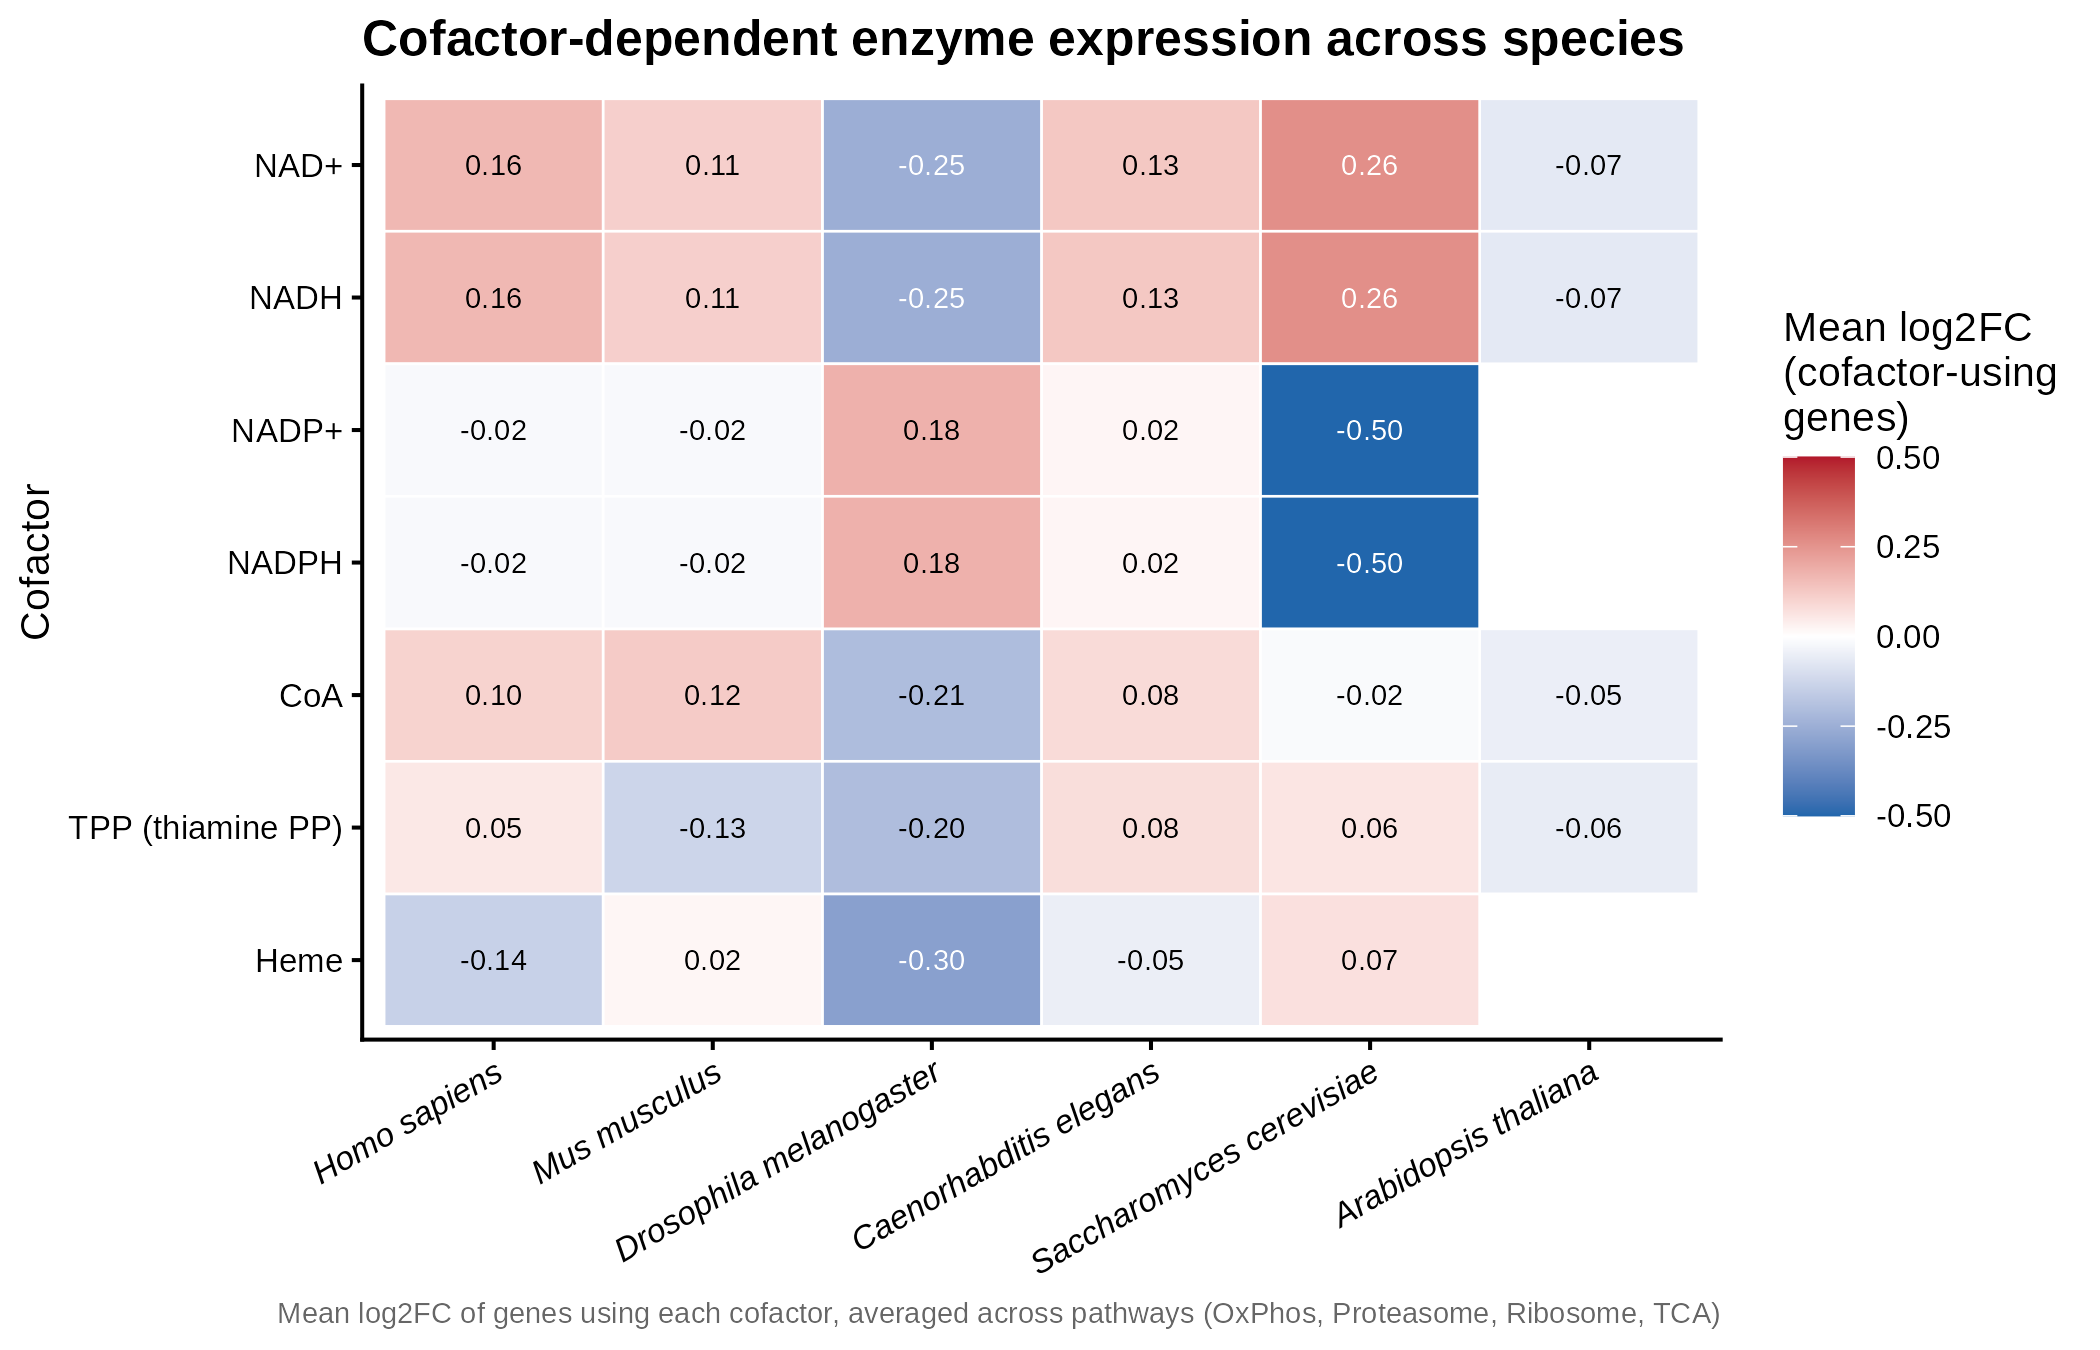
\includegraphics[width=0.9\textwidth]{fig7_cofactor_summary.png}
    \caption{
        \textbf{Cofactor-gene enrichment summary.}
        Bar plot showing mean $\log_2$(FC) of genes involved in the biosynthesis or 
        utilization of 12 enzyme cofactors across the six species. Error bars represent 
        $\pm 1$ SD. NAD+, NADH, FAD, and heme-related genes show significant, consistent 
        downregulation (blue), supporting the hypothesis of reduced aerobic capacity.
    }
    \label{fig:fig7}
\end{figure}

% ---
% DISCUSSION
% ---
\section{Discussion}
\label{sec:discussion}

This cross-species meta-analysis reveals a striking conservation in the spaceflight 
transcriptomic response: coordinated downregulation of mitochondrial genes across 
six eukaryotic organisms spanning more than a billion years of evolutionary divergence. 
This finding challenges the assumption that organismal responses to spaceflight are 
primarily species-, tissue-, or mission-specific phenomena, and instead suggests that 
mitochondrial metabolic suppression represents a fundamental, systems-level adaptation 
to microgravity stress.

\subsection{Evolutionary conservation of the spaceflight response}
\label{sec:discussion:evolution}

The conservation of mitochondrial suppression across \textit{Homo sapiens}, \textit{Mus musculus}, 
\textit{Drosophila melanogaster}, \textit{Caenorhabditis elegans}, \textit{Saccharomyces cerevisiae}, 
and \textit{Arabidopsis thaliana} is remarkable given the vast evolutionary distances 
between these organisms and the differences in their native habitats and physiology. 
None of these species has been subject to strong selection pressure for spaceflight 
adaptation in their recent evolutionary history. The conservation therefore likely 
reflects a general stress-response program—possibly orthologous to responses to 
hypoxia, nutrient limitation, or other physiological challenges.

\subsection{Mechanistic hypotheses: Metabolic suppression and oxidative stress}
\label{sec:discussion:mechanism}

We propose two non-exclusive mechanisms for this conserved mitochondrial suppression:

\textbf{(1) Metabolic reprogramming to reduce oxidative stress.} Spaceflight combines 
multiple stressors—microgravity, radiation, and altered circadian rhythms—that can 
increase mitochondrial reactive oxygen species (ROS) production. By downregulating 
oxidative phosphorylation and energy metabolism, organisms may reduce both ROS production 
and the accumulation of damage. This strategy trades short-term ATP production for 
long-term cellular integrity.

\textbf{(2) Reduced energy demand in microgravity.} Muscle atrophy and reduced gravitational 
load on skeletal structures reduce the mechanical work required of cells, potentially 
lowering ATP demand. The observed downregulation of mitochondrial capacity may be a 
rational response to decreased energy requirements.

Both mechanisms are likely operative to varying degrees across tissues and species.

\subsection{Limitations and future directions}
\label{sec:discussion:limitations}

Our analysis, while comprehensive in its cross-species scope, faces several constraints:

\begin{enumerate}
    \item \textbf{Tissue heterogeneity:} Most datasets sampled whole tissues or organs, 
          which contain multiple cell types. Single-cell or cell-type-specific analysis 
          may reveal that suppression is concentrated in particular cell populations.
    
    \item \textbf{Post-transcriptomic layers:} We analyzed transcript abundance, which 
          does not necessarily reflect protein abundance or enzyme activity. Proteomic 
          and metabolomic studies are needed to confirm that reduced mitochondrial 
          transcription translates to reduced mitochondrial function.
    
    \item \textbf{Temporal resolution:} Most datasets sampled a single timepoint during 
          or shortly after spaceflight. Time-series studies might reveal dynamic shifts 
          in mitochondrial expression (e.g., initial suppression followed by recovery 
          or further decompensation).
    
    \item \textbf{Mission confounds:} Spaceflight missions vary in duration, vehicle 
          (ISS vs. spacecraft), crew size, and other factors. While we modeled these as 
          covariates where possible, a larger dataset collection might enable more 
          granular phenotyping.
\end{enumerate}

Future work should integrate proteomic, metabolomic, and single-cell transcriptomic 
data from spaceflight experiments; develop model organisms (e.g., \textit{Drosophila} 
or \textit{C. elegans}) optimized for spaceflight research; and conduct ground-based 
studies (e.g., simulated microgravity via clinorotation) to validate mechanistic 
hypotheses.

\subsection{Implications for space exploration and human health}
\label{sec:discussion:implications}

The conserved downregulation of mitochondrial metabolism in spaceflight may have 
important implications for long-duration spaceflight and human colonization of the Moon 
and Mars. Impaired mitochondrial function could contribute to muscle atrophy, bone loss, 
immune dysfunction, and accelerated aging observed in astronauts. Conversely, 
understanding the molecular basis of this adaptive response might reveal therapeutic 
targets for Earth-based conditions characterized by mitochondrial dysfunction or 
accelerated aging (e.g., sarcopenia, neurodegeneration).

Pharmaceutical or genetic interventions that preserve mitochondrial capacity in 
spaceflight might improve crew health and performance during long-duration missions. 
Conversely, transiently enhancing mitochondrial suppression (e.g., via caloric 
restriction or pharmacological interventions) might protect against radiation and 
oxidative stress during high-radiation transit phases.

% ---
% METHODS
% ---
\section{Methods}
\label{sec:methods}

\subsection{Data acquisition}
\label{sec:methods:acquisition}

We queried the NASA OSDR Biological Data API 
(\url{https://visualization.osdr.nasa.gov/biodata/api/v2/query/}) to enumerate 
RNA-seq and microarray datasets with spaceflight factors across six eukaryotic 
species. Final dataset selection comprised 22 studies: 7 mouse, 4 human, 3 
\textit{Arabidopsis}, 3 fly, 4 worm, and 1 yeast. Processed data (DE tables, 
count matrices, sample tables) were downloaded via the OSDR web API.

\subsection{Differential expression analysis}
\label{sec:methods:de}

For 19 of 22 datasets, we used GeneLab Research Community Portal (RCP) pre-computed 
DE tables (DESeq2 for RNA-seq; limma for microarray). For three datasets lacking 
pre-computed DE (OSD-96 fly, OSD-35 worm), we performed de novo differential expression 
analysis using DESeq2 and limma respectively. We selected contrasts where the only 
difference between groups was spaceflight vs. ground control, and applied tiered 
statistical thresholds (standard: padj $< 0.05$, $|\log_2\text{FC}| > 1$; relaxed 
padj $< 0.10$, $|\log_2\text{FC}| > 0.5$ for low-power datasets; nominal $p < 0.05$, 
$|\log_2\text{FC}| > 0.5$ for datasets without replicates).

\subsection{Orthology mapping}
\label{sec:methods:orthology}

We constructed a human-anchored orthology matrix using OrthoDB v12 (bulk downloads 
from \url{https://data.orthodb.org/v12/download/odb_data_dump/}) and babelgene 
(v0.99.7). For \textit{Arabidopsis}, we mapped TAIR IDs to human orthologs via 
OrthoDB eukaryota-level ortholog groups. The final matrix contains 51,474 
ortholog pairs covering 18,030 human genes.

\subsection{Subcellular compartment assignment}
\label{sec:methods:compartment}

We performed Gene Ontology Cellular Component (GO CC) enrichment per species using 
clusterProfiler's \texttt{enrichGO} (Benjamini-Hochberg correction, $p < 0.05$). 
All enriched GO CC terms were manually classified into 16 organelle categories based 
on biological knowledge and term definitions.

\subsection{Cross-species meta-analysis}
\label{sec:methods:meta}

For each organelle category, we applied Fisher's combined probability test on 
per-species $p$-values for all orthologs tested in each species. A gene was called 
``conserved'' if Fisher FDR $< 0.05$, the gene was significant (DEG) in $\geq 3$ 
species, and direction was consistent ($\geq 80\%$ of significant species in the 
same direction).

\subsection{Pathway and cofactor analysis}
\label{sec:methods:pathway}

We fetched KEGG pathway-gene links via the KEGG REST API for four pathways enriched 
in the conserved-suppressed gene set (hsa00020, hsa00190, hsa03010, hsa03050). 
Pathway genes were mapped to per-species log$_2$(FC) values and visualized using 
ggkegg (v1.11.0). For cofactor analysis, we mapped 14 cofactors to human genes via 
KEGG compound → reaction → enzyme → gene chains.

\subsection{Visualization}
\label{sec:methods:viz}

All figures use a viridis-based colorblind-friendly palette with fixed species colors. 
SVG and PNG (300 dpi) formats were generated in R using ggplot2, ComplexHeatmap, and 
ggkegg packages. Complete code is available in the repository's \texttt{scripts/} folder.

% ---
% ACKNOWLEDGMENTS
% ---
\section*{Acknowledgments}

We thank the NASA OSDR team and all contributing research groups for making their 
spaceflight transcriptomic datasets publicly available. We acknowledge the use of 
OrthoDB v12 and KEGG databases for orthology and pathway resources. This work was 
assisted by Biomni (Phylo AI) for data analysis scripting and visualization.

% ---
% COMPETING INTERESTS
% ---
\section*{Competing interests}

The authors declare no competing financial interests.

% ---
% AUTHOR CONTRIBUTIONS
% ---
\section*{Author contributions}

R.B. conceived the study, performed the meta-analysis, generated figures, and wrote 
the manuscript. [Additional author contributions to be added upon finalization.]

% ---
% DATA AVAILABILITY
% ---
\section*{Data availability}

All input datasets are publicly available via the NASA OSDR 
(\url{https://osdr.nasa.gov}). Supplementary tables, orthology matrices, and 
enrichment results are deposited on Zenodo [DOI to be assigned]. Analysis code 
and figure-generation scripts are available at 
\url{https://github.com/dr-richard-barker/OSDR_X-species_V2}.

% ---
% BIBLIOGRAPHY
% ---
\newpage
\printbibliography

% ---
% SUPPLEMENTARY INFORMATION (optional sections follow)
% ---
\newpage
\appendix

\section{Supplementary Tables}
\label{sec:supp:tables}

\subsection*{Supplementary Table S1}
\label{sec:supp:table_s1}

Complete dataset inventory: OSDR accession, organism, platform, sample size, 
spaceflight duration, tissue, and DEG counts.

\subsection*{Supplementary Table S2}
\label{sec:supp:table_s2}

Orthology matrix: human gene ID, Ensembl ID, per-species orthologs, presence/absence 
in each species.

\subsection*{Supplementary Table S3}
\label{sec:supp:table_s3}

Gene Ontology Cellular Component (GO CC) enrichment results per species (all terms, 
FDR, gene counts).

\subsection*{Supplementary Table S4}
\label{sec:supp:table_s4}

GO CC terms manually classified into 16 organelle categories.

\subsection*{Supplementary Table S5}
\label{sec:supp:table_s5}

Per-species differential expression table for all 18,030 human-anchored orthologs 
(log$_2$ FC, padj, direction consistency flag).

\subsection*{Supplementary Table S6}
\label{sec:supp:table_s6}

Fisher's combined test results for all organelle-ortholog associations (Fisher $p$, 
FDR, direction, count of significant species).

\subsection*{Supplementary Table S7}
\label{sec:supp:table_s7}

Complete list of 49 conserved mitochondrial-suppressed orthologs with per-species 
fold changes and pathway assignments.

\subsection*{Supplementary Table S8}
\label{sec:supp:table_s8}

KEGG pathway gene lists with per-species and meta-analytic log$_2$ FC values 
(pathways hsa00020, hsa00190, hsa03010, hsa03050).

\subsection*{Supplementary Table S9}
\label{sec:supp:table_s9}

Cofactor-gene mapping: compound ID, cofactor name, associated genes, per-species 
log$_2$ FC.

\end{document}
